\chapter{Capacitively Coupled Pixel Detectors for the CLIC Vertex Detector}
\label{chap:clicvertex}

\chapterquote{The beginning of wisdom is this: Get wisdom.  Though it cost all you have, get understanding.}
{Proverbs 4:7}

%========================================================================================
%========================================================================================

\section{Introduction}

Identification of heavy-flavour quarks and tau-leptons at any of the currently proposed linear collider experiments will rely upon precise reconstruction of secondary displaced vertices that are produced when these particles decay \cite{Linssen:2012hp}.  Furthermore, the ability to accurately associate any daughter tracks produced in such decays to the secondary vertices is essential.  At CLIC, this can only be realised using a vertex detector with a very high spatial resolution, of approximately 3~${\micro}$m, and good geometric coverage, extending to low polar angles $\theta$.  The vertex detector must also have a low material budget (less than 0.2~\%~$\text{X}_{0}$ per layer) in order to prevent additional decay vertices from material interactions, and allow efficient track reconstruction despite the high presence of beam-induced background particles.  Tracking in the vertex detector will be aided by the use of time-stamping of individual hits, to an accuracy of 10~ns, to identify particles produced from the physics event of interest.  

As there are currently no technology options that fulfil all of the criteria for the CLIC vertex detector, the CLIC experiment has developed an extensive R\&D program where new technologies for the vertex detector are considered.  High-voltage complementary metal-oxide-semiconductor (HV-CMOS) sensors, which are capacitively coupled to a separate readout application-specific integrated circuit (ASIC) are one such option. The performance of prototype detectors based upon this technology and the impact of mechanical tolerances present in their manufacture are presented in this chapter.  

%========================================================================================

\subsection{HV-CMOS}
Pixel detectors can be broadly classified in two groups: hybrid detectors, where a separate sensor and readout chip are bonded together; and fully-integrated devices, where the collection diode is implanted in the same piece of silicon as the readout circuitry.  Fully-integrated devices have traditionally not been suitable for applications with high timing requirements due to the relatively slow charge collection time and limited on-pixel functionality.  However, recent developments in CMOS technologies \cite{Weste:2010:CVD:1841628} have led to new detector designs that may overcome some of these issues. 

HV-CMOS is a processing technology whereby the n-MOS and p-MOS transistors forming the on-pixel electronics are placed entirely within a deep n-well, as shown in figure \ref{fig:hvcmos}.  By varying the voltage applied at the gate terminal, n-MOS and p-MOS transistors are able to control the current flowing between the source and drain terminals.  The gate voltage produces an inversion layer between the source and drain terminals that acts as a conduit, allowing current to flow between the source and drain as shown in figure \ref{fig:nmos}.  The voltage at the gate, with respect to the body, controls the width of the inversion layer and hence the magnitude of this current.  Logic operations can be performed directly on-pixel using various configurations of n-MOS and p-MOS transistors.

\begin{figure}[h!]
\centering
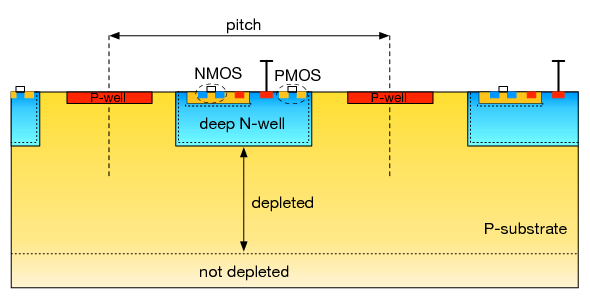
\includegraphics[width=0.75\textwidth]{CLICdpVertex/Plots/HV-CMOSDiagram.png}
\caption[Schematic cross section of an HV-CMOS sensor: the deep n-well is the charge-collecting electrode and also contains additional CMOS circuitry such as a preamplifier.  Image taken from \cite{Benoit:2016vup}.]{Schematic cross section of an HV-CMOS sensor: the deep n-well is the charge-collecting electrode and also contains additional CMOS circuitry such as a preamplifier.  Image taken from \cite{Benoit:2016vup}.}\micro
\label{fig:hvcmos}
\end{figure}

\begin{figure}[h!]
\centering
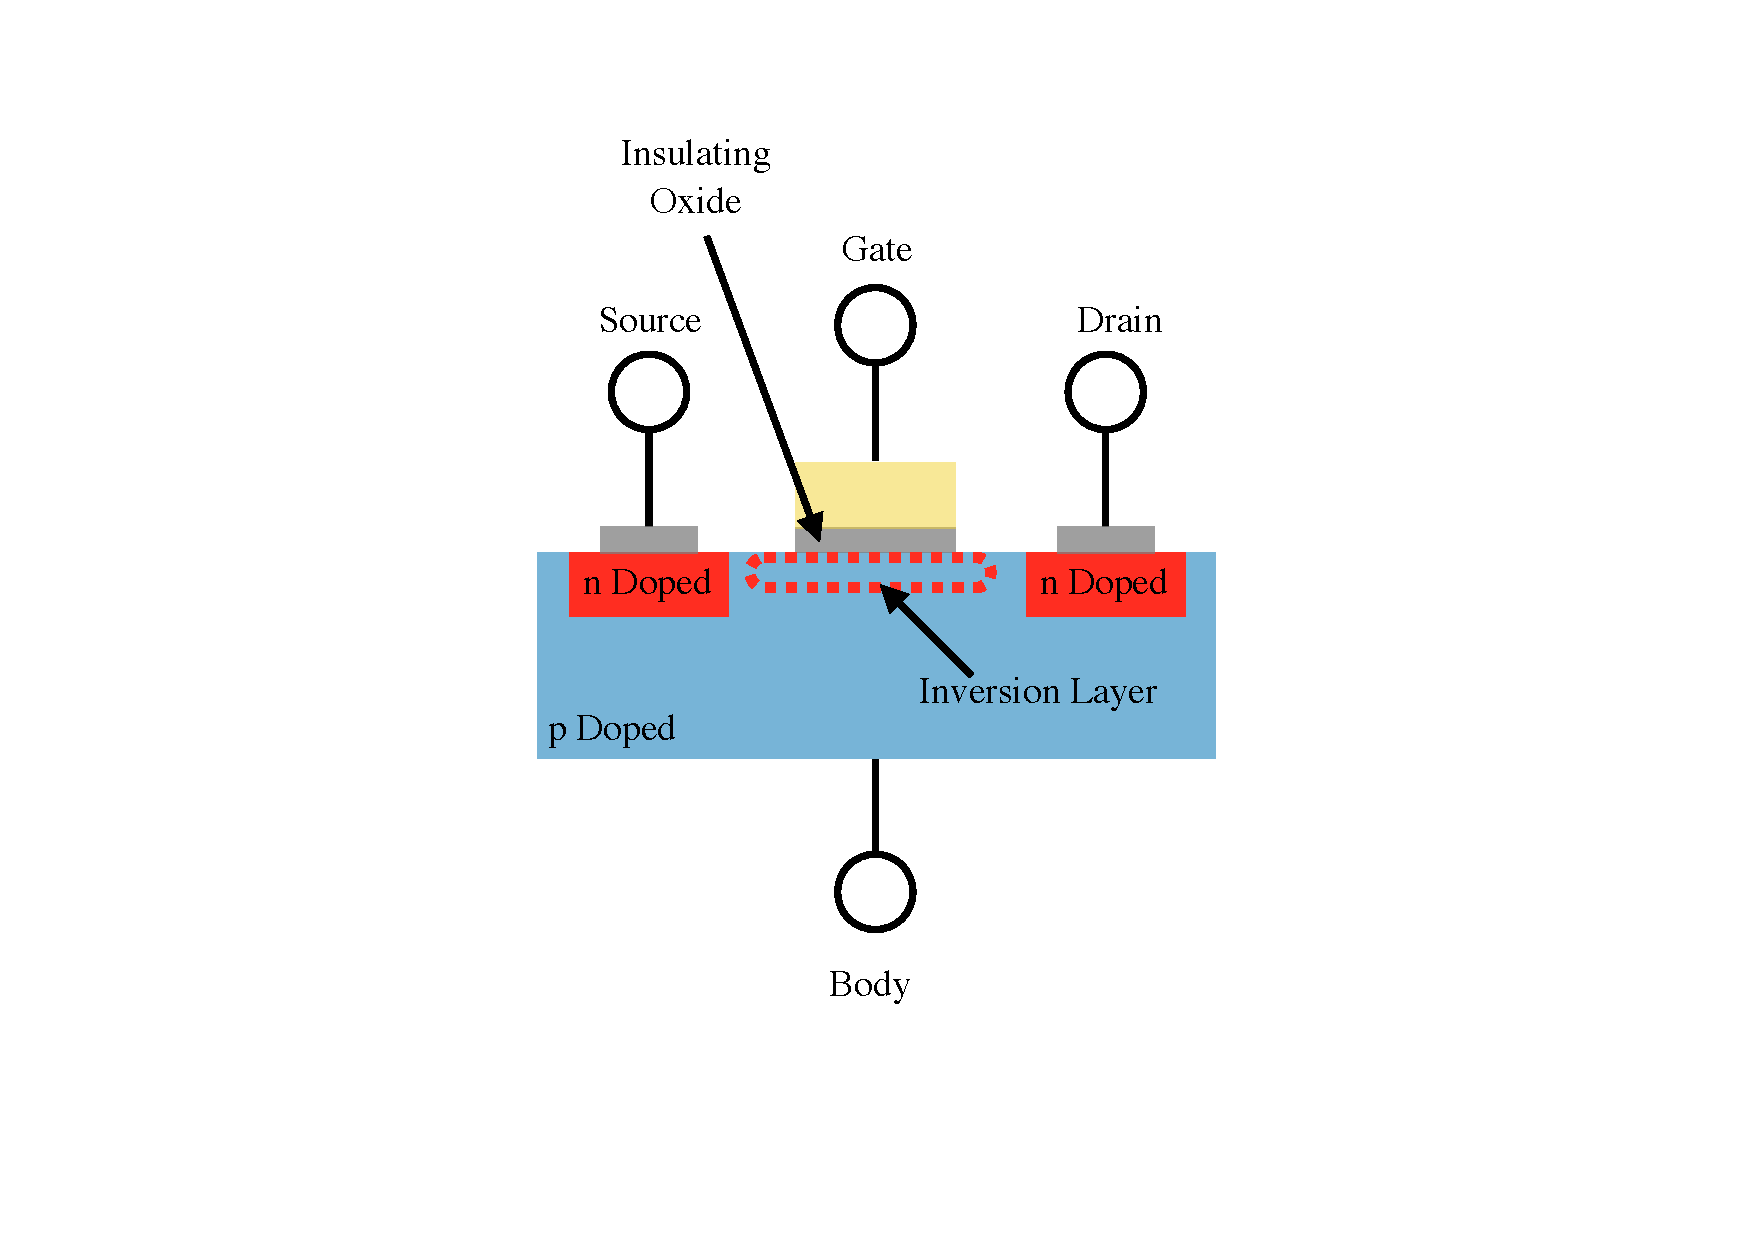
\includegraphics[width=0.5\textwidth]{CLICdpVertex/Plots/FETDiagram.pdf}
\caption[Schematic cross section of an n-MOS transistor.  p-MOS transistors have a similar cross section where the n and p doped regions are switched.]{Schematic cross section of an n-MOS transistor.  p-MOS transistors have a similar cross section where the n and p doped regions are switched.}
\label{fig:nmos}
\end{figure}

For the HV-CMOS, the deep n-well housing the on-pixel electronics acts as the charge collection diode as well as shielding the circuitry from the p-substrate.  This shielding allows for the application of a moderate bias voltage to the sensor bulk that produces a depletion region, which facilitates fast charge collection via a drift current.  In contrast, traditional monolithic active pixel sensors (MAPS) have a much smaller depletion region meaning charge collection occurs primarily through the slower mechanism of diffusion.  Furthermore, in conventional MAPS there is potential for competition in charge collection between the n-well collecting diode and the p-MOS transistors used to perform logic operations since the p-MOS transistors are embedded within an n-well.  This only occurs as the n-well collection diode is separated from the n-wells housing the p-MOS transistors.  HV-CMOS technology does not suffer from this issue as the deep n-well collecting diode houses the p-MOS transistors, meaning charge is only collected at a single well in the sensor bulk.  

HV-CMOS technology thus offers the possibility of fast charge collection with integrated on-pixel functionality, but several limitations still exist.  As the on-pixel electronics have to be placed inside the deep n-well and the n-wells of neighbouring pixels have to be isolated from each other, there is a limited physical area of the pixel that can be used for transistor layout, which limits the available on-pixel functionality.  In addition to this, it is not possible to implement full CMOS logic inside the deep n-well as coupling between p-MOS transistors and the collection diode will lead to noise injection at the charge collection node.  While it is possible to embed p-MOS transistors within a p-well to shield them from the deep n-well, so-called "quadruple-well technology", to give access to full CMOS logic this option is not readily available for prototyping.  By restricting the complexity of on-pixel electronics and using a separate readout ASIC, it is possible to overcome many of these issues.  When coupled with the fast charge collection time and removal of competition in charge collection, this makes HV-CMOS technology highly desirable for use in the CLIC vertex detector.

%========================================================================================

\subsection{CLIC ASICs}
As HV-CMOS technology is such a promising option for use at the CLIC vertex detector, prototype devices based on this technology have been developed for testing.  Two ASICs have been developed: the capacitively coupled pixel detector version 3 (CCPDv3), a sensor chip based on HV-CMOS technology, and the CLICpix, a readout chip providing additional on-pixel logic operations.  The pixel pitch of the chips, both the CCPDv3 and the CLICpix, is 25~${\micro}$m, which should be sufficient to meet the requirements for the CLIC vertex detector.  Each of the prototype ASICs consists of a matrix of 64$\times$64 pixels.  The CCPDv3 is fabricated in a 180~nm HV-CMOS process, where 180~nm refers to the smallest size building block that can be used for creating the integrated circuits on a silicon wafer.  This is comparable to device fabrication at the LHC, which typically uses a 130 and/or 250~nm CMOS processes \cite{Aaij:2244311, Dominguez:1481838}.  In comparison, the CLICpix is fabricated in a 65~nm process, which makes it possible to have more complex on-pixel circuitry incorporated into it than would be possible in previous generations of pixel detectors.  A schematic of these devices can be found in figure \ref{fig:ccpdandclicpix}.  

\begin{figure}[h!]
\centering
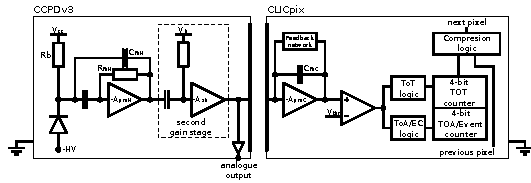
\includegraphics[width=1.0\textwidth]{CLICdpVertex/Plots/schematic.pdf}
\caption[Schematic of CCPDv3 and CLICpix pixels. Figure taken from \cite{FabricationNote}.]{Schematic of CCPDv3 and CLICpix pixels. Figure taken from \cite{FabricationNote}.}
\label{fig:ccpdandclicpix}
\end{figure}

%========================================================================================

\subsubsection{CLICpix}

CLICpix is a hybrid pixel readout chip that has been developed for the CLIC vertex detector. Each CLICpix pixel contains a charge-integrating amplifier connected to a discriminator, as shown in figure \ref{fig:ccpdandclicpix}.  The discriminator remains high for as long as the input signal is over a given threshold, and this output is then used as the input for further logic operations.  The additional logic operations record the time of arrival and magnitude of the collected charge, using a Time over Threshold (ToT) measurement. The ToT is stored in a 4-bit on-pixel counter.  

The CLICpix operates using a shutter-based readout, where the entire matrix is kept active while the shutter is open and when closed the matrix is read out in its entirety.  This is designed to match the expected beam structure for the CLIC experiment, as the accelerator will deliver bunch trains of $e^{+}$ and $e^{-}$ that are separated by 20~ms.  Each bunch train contains 312~bunches with a spacing of 0.5~ns, giving a total train length of 156~ns.  Furthermore, the shutter-based readout is well suited to power-pulsing, where the power to the front-end electronics is turned off between bunch crossings.  This helps to significantly reduce the power consumption of the detector.

The threshold voltage, the voltage required for the discriminator to register an output, seen by each CLICpix pixel is slightly different due to variations in the manufacturing process.  If these variations are not accounted for then the behaviour of the device across the matrix will not be uniform.  To minimise the impact of these fluctuations, each CLICpix pixel contains a 4-bit local adjustment to the threshold voltage, which is calibrated to unify the response across the matrix.  The threshold "equalisation" is achieved by performing two threshold scans across the matrix, once with all four bits set to 0 (no local threshold adjustment), and a second time with all four bits set to 1 (maximum local threshold adjustment).  For each scan, the baseline voltage of each pixel is determined. By applying a linear interpolation between the 0000 and 1111 cases, each pixel can be tuned to a common point, such that all pixels respond at the same global threshold.

%========================================================================================

\subsection{Capacitive Coupling}

Solder bump-bonding is typically used to connect the sensor and readout ASIC in hybrid pixel detectors.  This procedure uses small spheres of solder to connect each pixel on the sensor to the corresponding pixel on the readout ASIC.  There are several drawbacks to the use of this procedure for pixel detectors: it is expensive and sets limits on the thickness of both ASICs that is required for mechanical stability.  An alternative procedure for connecting the sensor and readout ASICs involves using a thin layer of glue to form a capacitive connection between the two.  This procedure reduces the cost and material budget with respect to bump-bonding, making it highly desirable for use in the CLIC vertex detector. In order to make this viable, it is necessary to implement an amplifier in the CCPDv3 pixel, shown in figure \ref{fig:ccpdandclicpix}, to boost the signal and overcome the intrinsically small coupling capacitance. 

%========================================================================================
%========================================================================================

\section{Device Fabrication}

There are two issues related to device manufacture that have to be considered when using capacitive coupling to connect the sensor and readout ASIC: the uniformity of the glue layer and the spatial alignment of the sensor and readout pads.  The former has been investigated in \cite{FabricationNote}, while the latter is the focus of this study.  In order to characterise the impact on detector performance of any misalignment between the CCPDv3 and the CLICpix pads, a number of assemblies have been constructed that purposefully contain misalignments, as shown in figure \ref{fig:alignment}.  Table \ref{table:alignment} contains a summary of the samples produced.

\begin{figure}[h!]
\centering
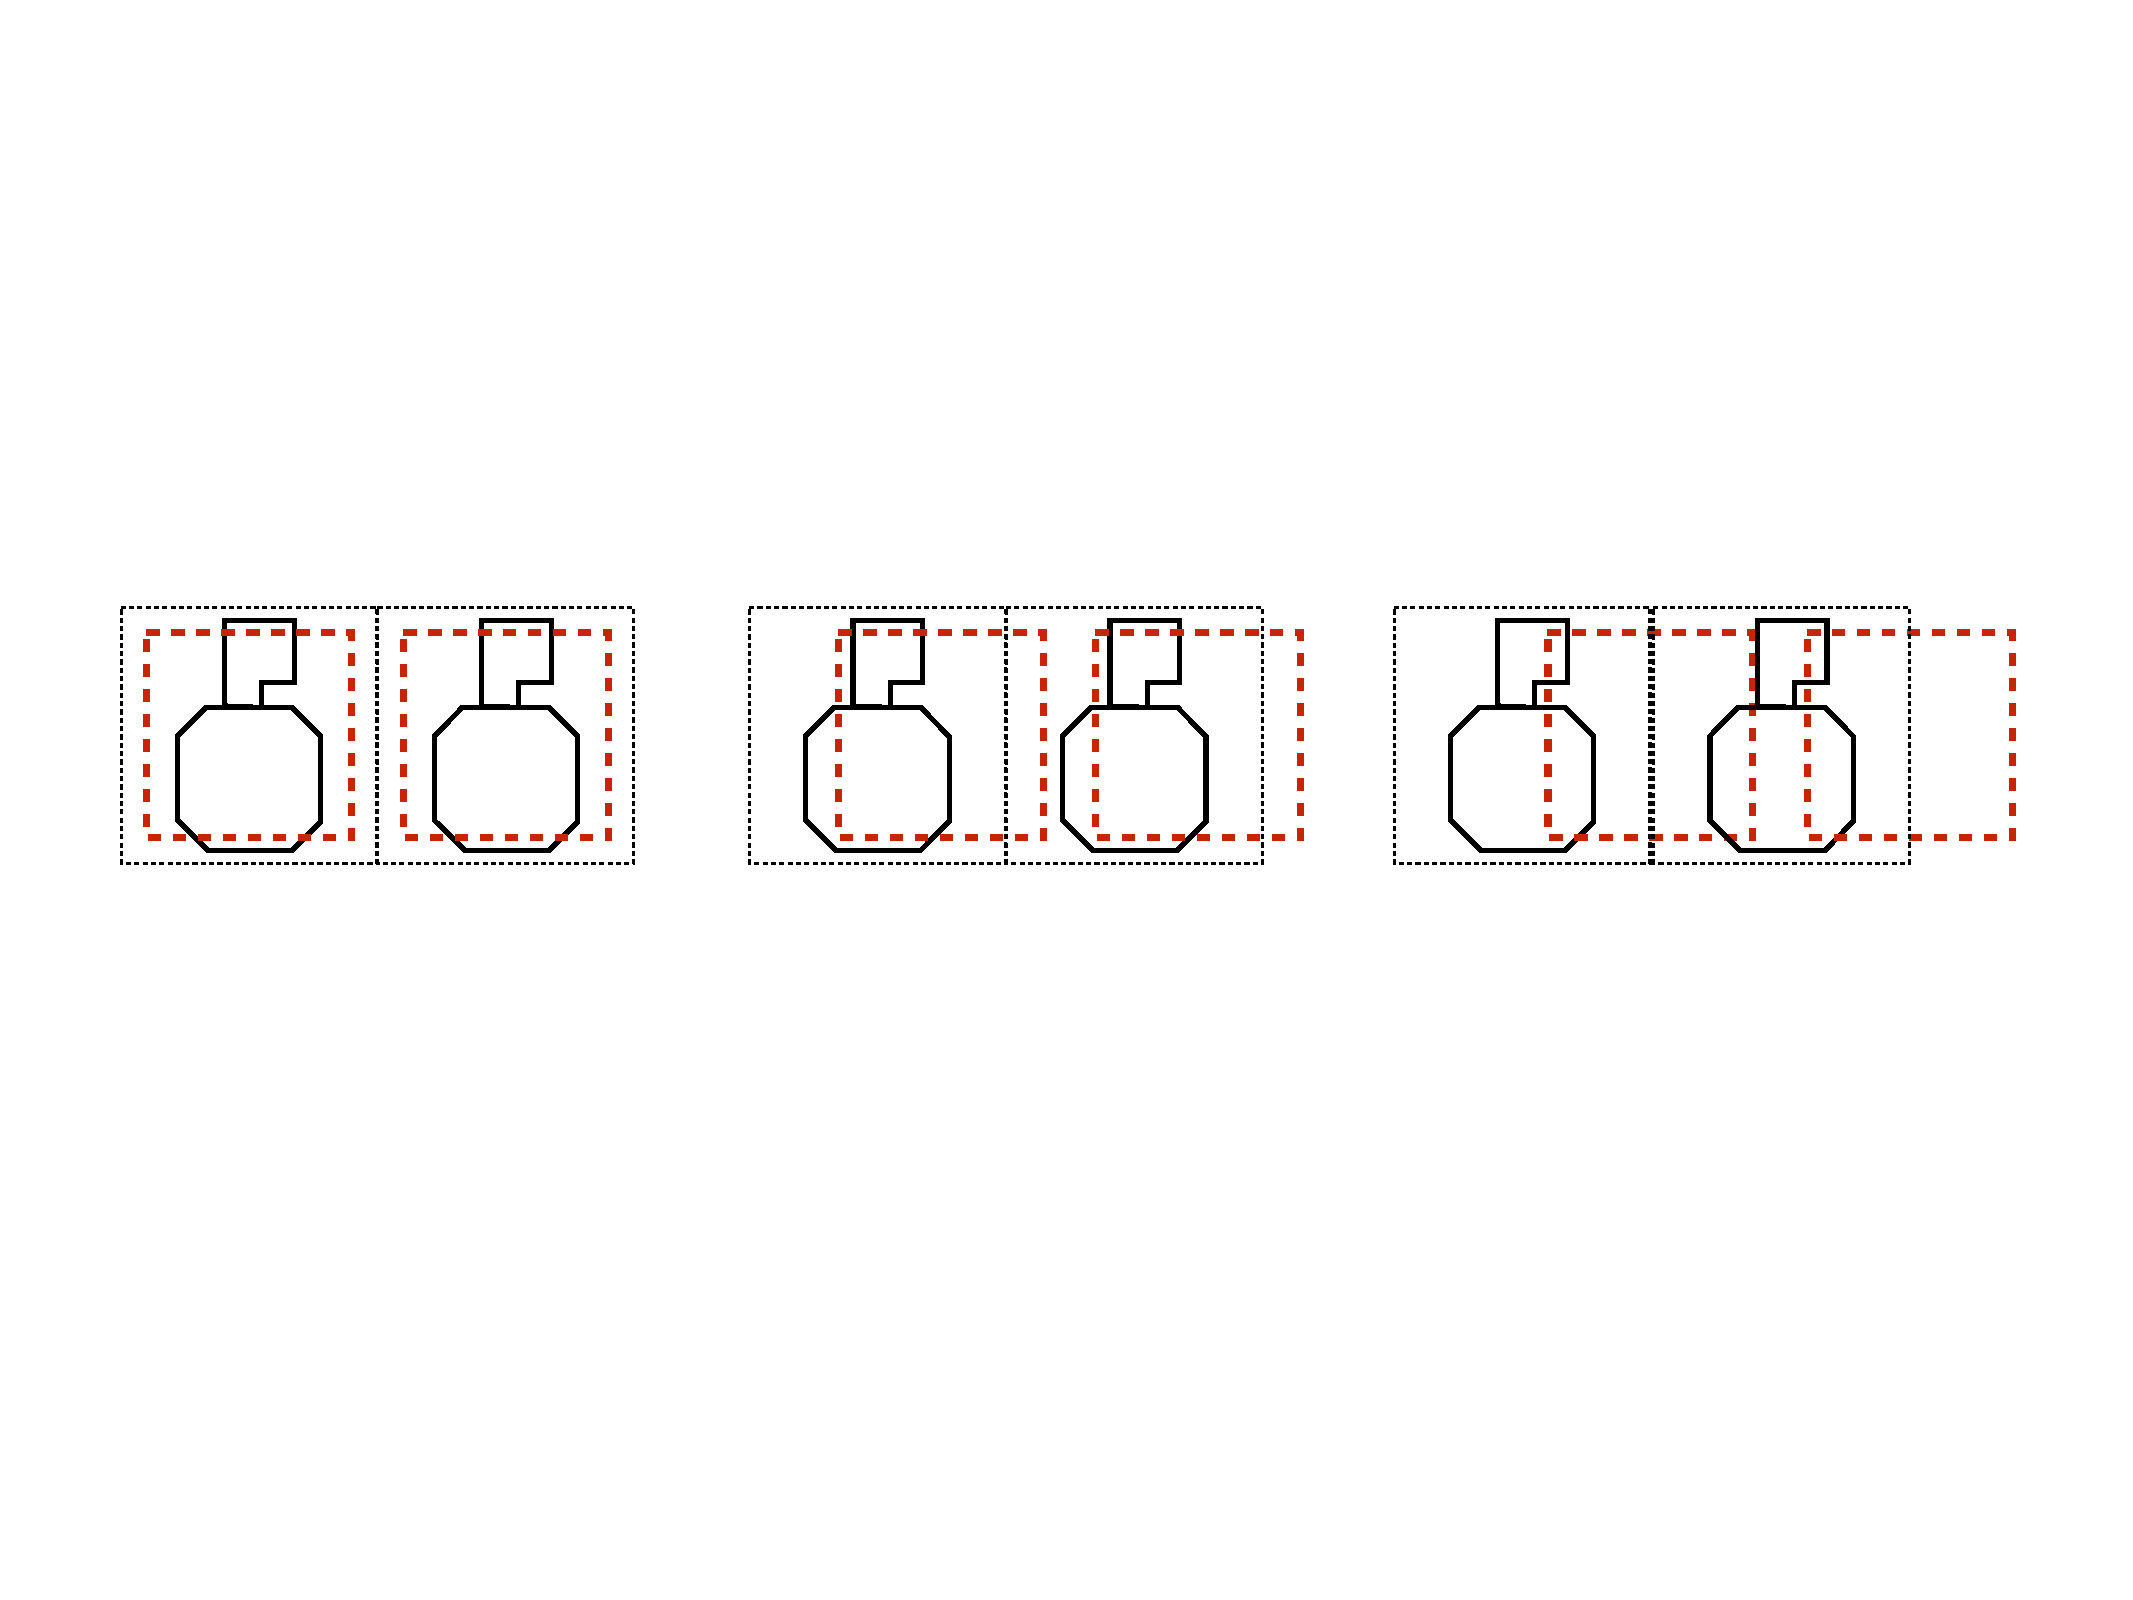
\includegraphics[width=1.0\textwidth]{CLICdpVertex/Plots/misalignedPads.pdf}
\caption[Alignment schematic of the CCPDv3 and CLICpix detectors studied.  The red dotted line represents the CCPDv3 pad and the solid black line represents the CLICpix top metal layer.  From left to right; centred pixels, 1/4 offset (6.25~${\micro}$m) and 1/2 offset (12.5~${\micro}$m).]{Alignment schematic of the CCPDv3 and CLICpix detectors studied.  The red dotted line represents the CCPDv3 pad and the solid black line represents the CLICpix top metal layer.  From left to right; centred pixels, 1/4 offset (6.25~${\micro}$m) and 1/2 offset (12.5~${\micro}$m).}
\label{fig:alignment}
\end{figure}

\begin{table}[h!]
\centering
\begin{tabular}{ l l }
\hline
Assembly & Alignment \\ 
\hline
SET 9 & Centred \\
SET 10 & $\frac{1}{4}$ Offset \\
%SET 11 & $\frac{1}{2}$ Offset \\
SET 12 & Centred \\
SET 13 & Centred \\
%SET 14 & $\frac{1}{2}$ Offset REMOVED, NO?\\
SET 15 & Centred \\
SET 16 & $\frac{1}{2}$ Offset \\
\hline
\end{tabular}
\caption[A list detailing the alignment of the CCPDv3 and CLICpix coupling pads for the devices considered in this study.]{A list detailing the alignment of the CCPDv3 and CLICpix coupling pads for the devices considered in this study.}
\label{table:alignment}
\end{table}

The full details of the glueing procedure can be found in \cite{FabricationNote}, along with a study of the absolute precision of the manufacturing procedure.  For devices constructed in an identical fashion to those considered here, the glue layer thicknesses were less than 1~${\micro}$m and the precision on the pad positioning was less than 2~${\micro}$m.  

%========================================================================================
%========================================================================================

\section{Device Characterisation}
A series of laboratory experiments were used to characterise the devices produced for this alignment study.  The devices were also tested in realistic experimental conditions using the CERN SPS test beam.  Due to the complexities of testing devices in a test beam, extensive laboratory tests were performed first to characterise as many properties of the assemblies as possible.  The laboratory experiments performed were:

\begin{itemize}
\item \textbf{Radioactive source measurements}.  The goal of this measurement is to measure the response of the CCPDv3 and CLICpix when a radioactive source is used to deposit charge within the CCPDv3 sensor.  
\item \textbf{Test pulse calibration of the CLICpix chip}.  The goal of this measurement is to calibrate the response of the CLICpix sensor.  This is achieved by examining the CLICpix response when injecting a quantity of charge directly into the input of the chip, which bypasses the CCPDv3 and glue layer.
\end{itemize} 

%========================================================================================

\subsection{Source Measurements}
\label{sec:source}
A radioactive source was used to deposit charge within the CCPDv3 sensor and the response of the CCPDv3 and CLICpix examined.  The CCPDv3 sensor converts the deposited charge into a voltage, which in turn passes through the capacitive glue layer and into the CLICpix chip.  Measurements were made of the output voltage produced by the CCPDv3 and the response of the CLICpix readout chip, in units of ToT.  As the exact amount of charge deposited by the radioactive source is unknown, calibration of the CCPDv3 is not possible.  Instead, this experiment focuses on examining the shape of the voltage produced by the CCPDv3 and determining the response of the CLICpix chip as a function of this voltage.  As the CCPDv3 signal passes through the capacitively coupled glue layer before entering the CLICpix chip, this study characterises the properties of the gluing layer as well as the sensor and readout chips.

%========================================================================================

\subsubsection{Experimental Setup}
The radioactive material used in this study was $\text{Sr}^{90}$.  $\text{Sr}^{90}$ undergoes $\beta^{-}$ decay to form $\text{Y}^{90}$, which in turn undergoes $\beta^{-}$ decay to form the stable isotope $\text{Z}^{90}$.  Each $\beta^{-}$ decay produces an $\text{e}^{-}$ and a $\bar{\nu}_{\text{e}}$, and the $\text{e}^{-}$ goes on to deposit charge in the CCPDv3 sensor.  The $\text{Sr}^{90}$ source used had an activity of 29.6 MBq.  

The radioactive source was positioned directly above the back-side of the CCPDv3 sensor, and measurements were made of both the ToT output from the CLICpix and the CCPDv3 analogue signal for individual pixels on the sensor.  The CCPDv3 pulse shape was recorded on a fast sampling oscilloscope that was also used to trigger the CLICpix readout.  The on-pixel event counter, which is located in the CLICpix chip, was used to veto events where multiple hits occurred within the active shutter period.  The CCPDv3 sensor was biased to 60~V during this experiment.  Examples of CCPDv3 output voltage pulses when using the $\text{Sr}^{90}$ source can be seen in figure \ref{fig:pulseshapes}.  The analogue output has a baseline voltage of $\approx 1.15$~V with signal saturation occurring around a height of 700~mV.  

\begin{figure}[h!]
\centering
\subfloat[]{\label{fig:pulseshape1}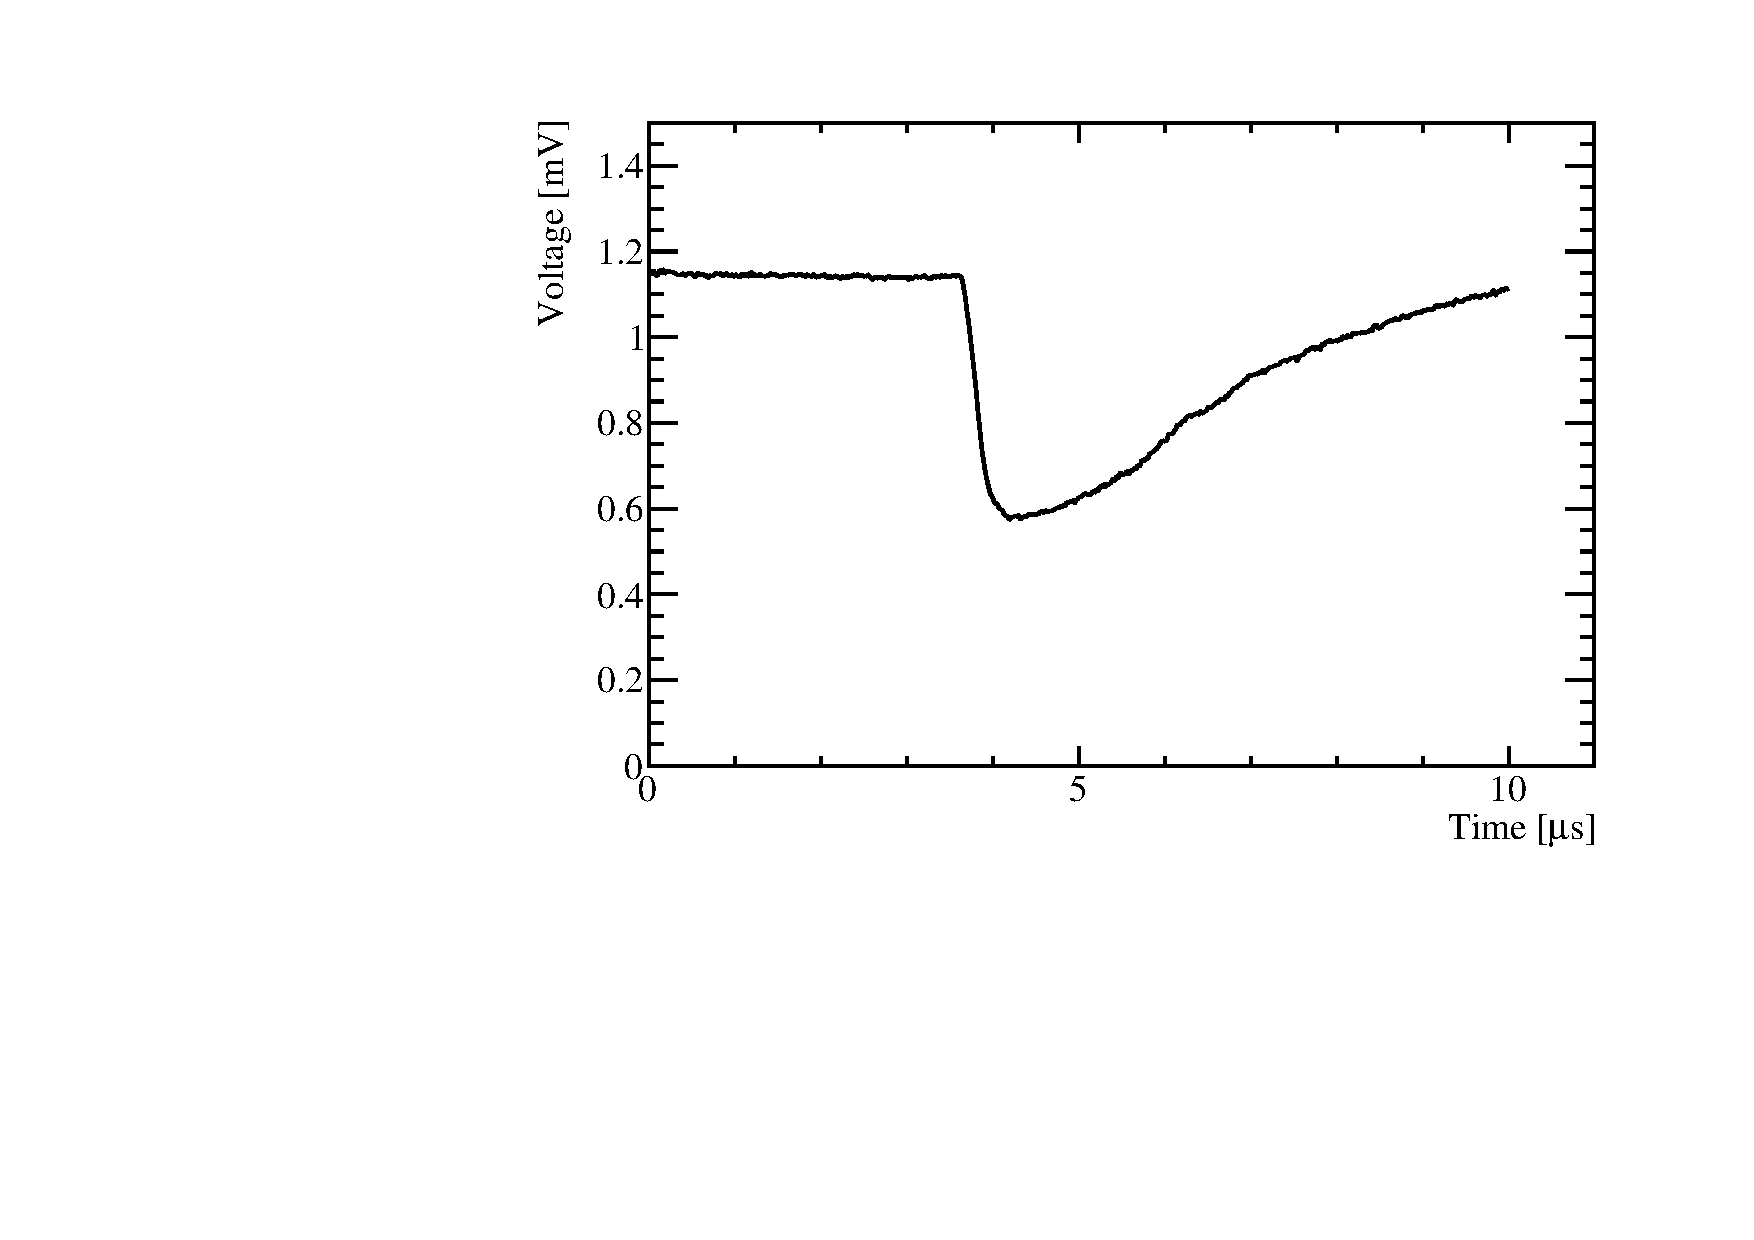
\includegraphics[width=0.5\textwidth]{CLICdpVertex/Plots/HV-CMOS/Frames/PulseShape01000NoOffset.pdf}}
\subfloat[]{\label{fig:pulseshape2}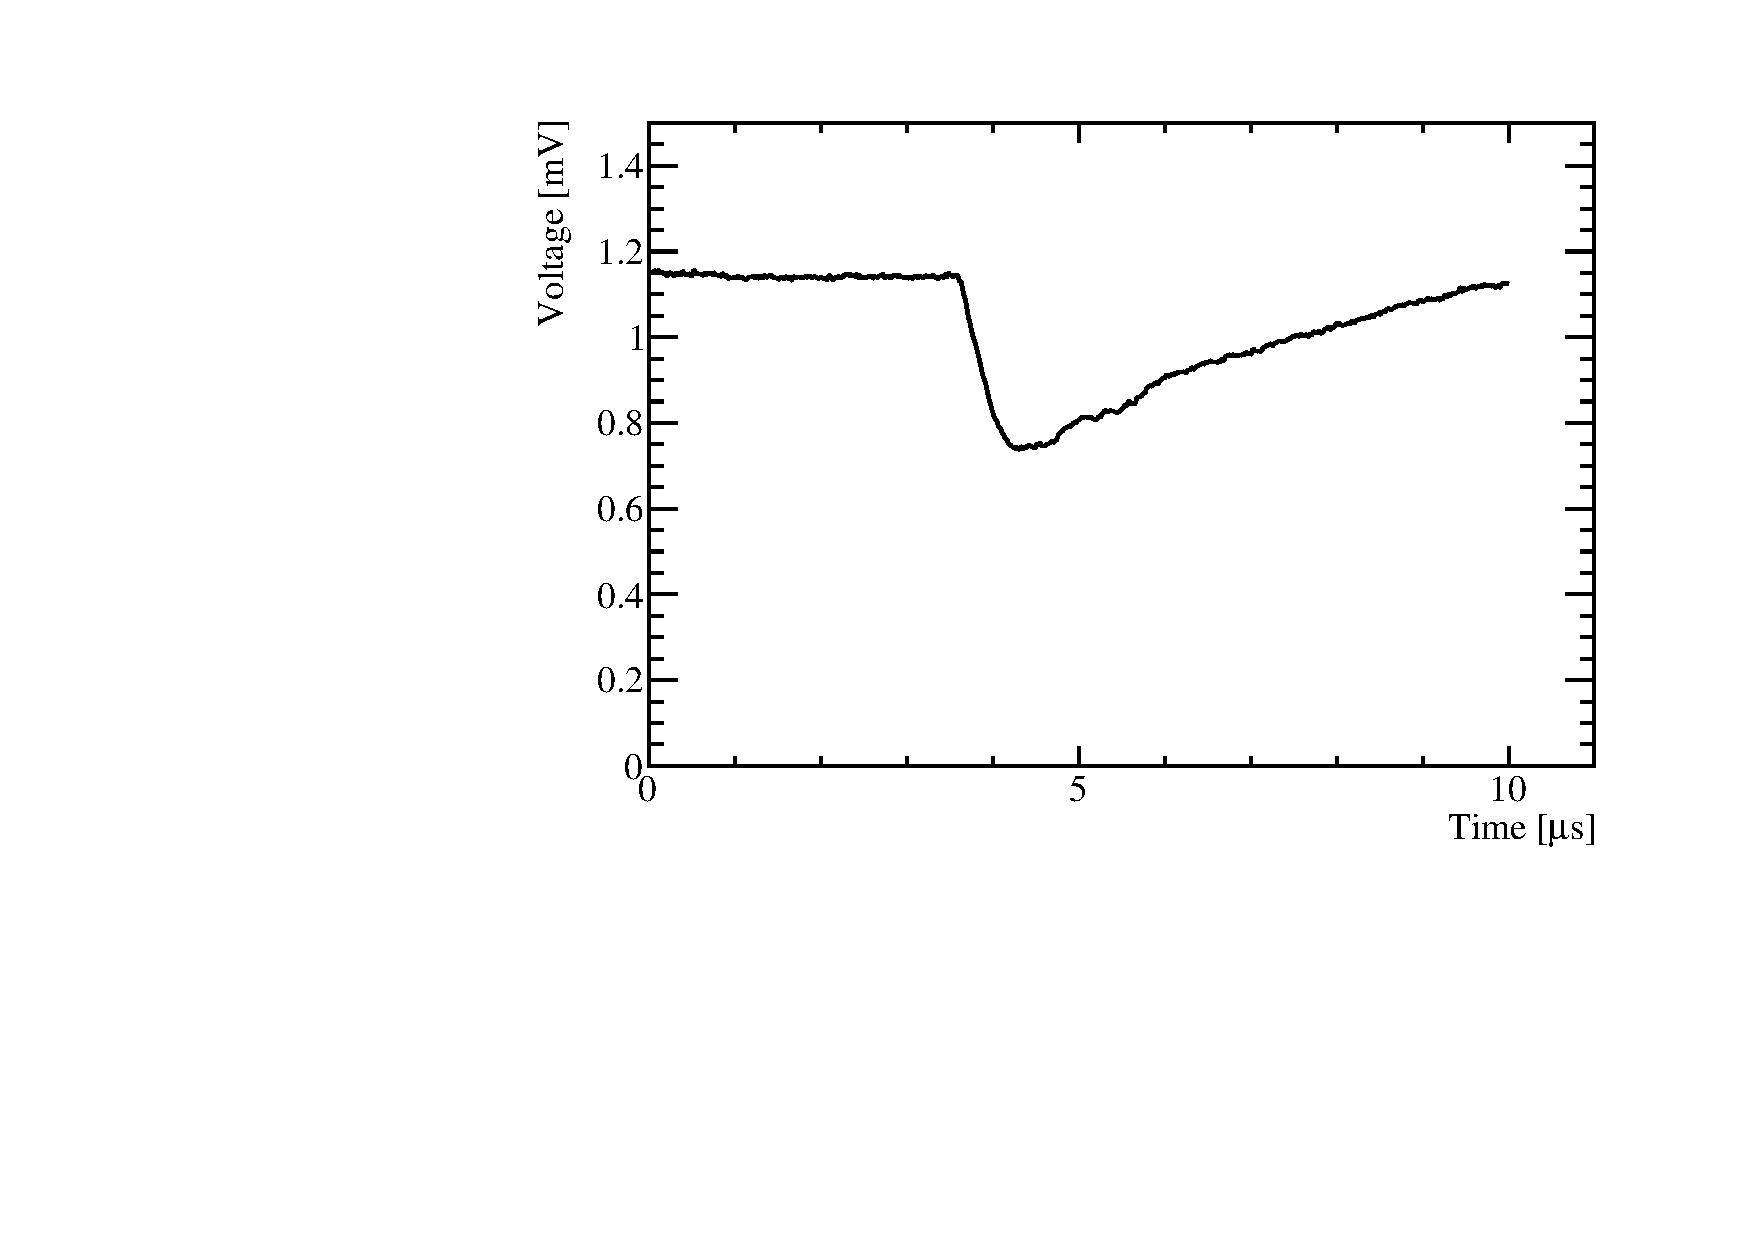
\includegraphics[width=0.5\textwidth]{CLICdpVertex/Plots/HV-CMOS/Frames/PulseShape01005NoOffset.pdf}}\hfill
\subfloat[]{\label{fig:pulseshape3}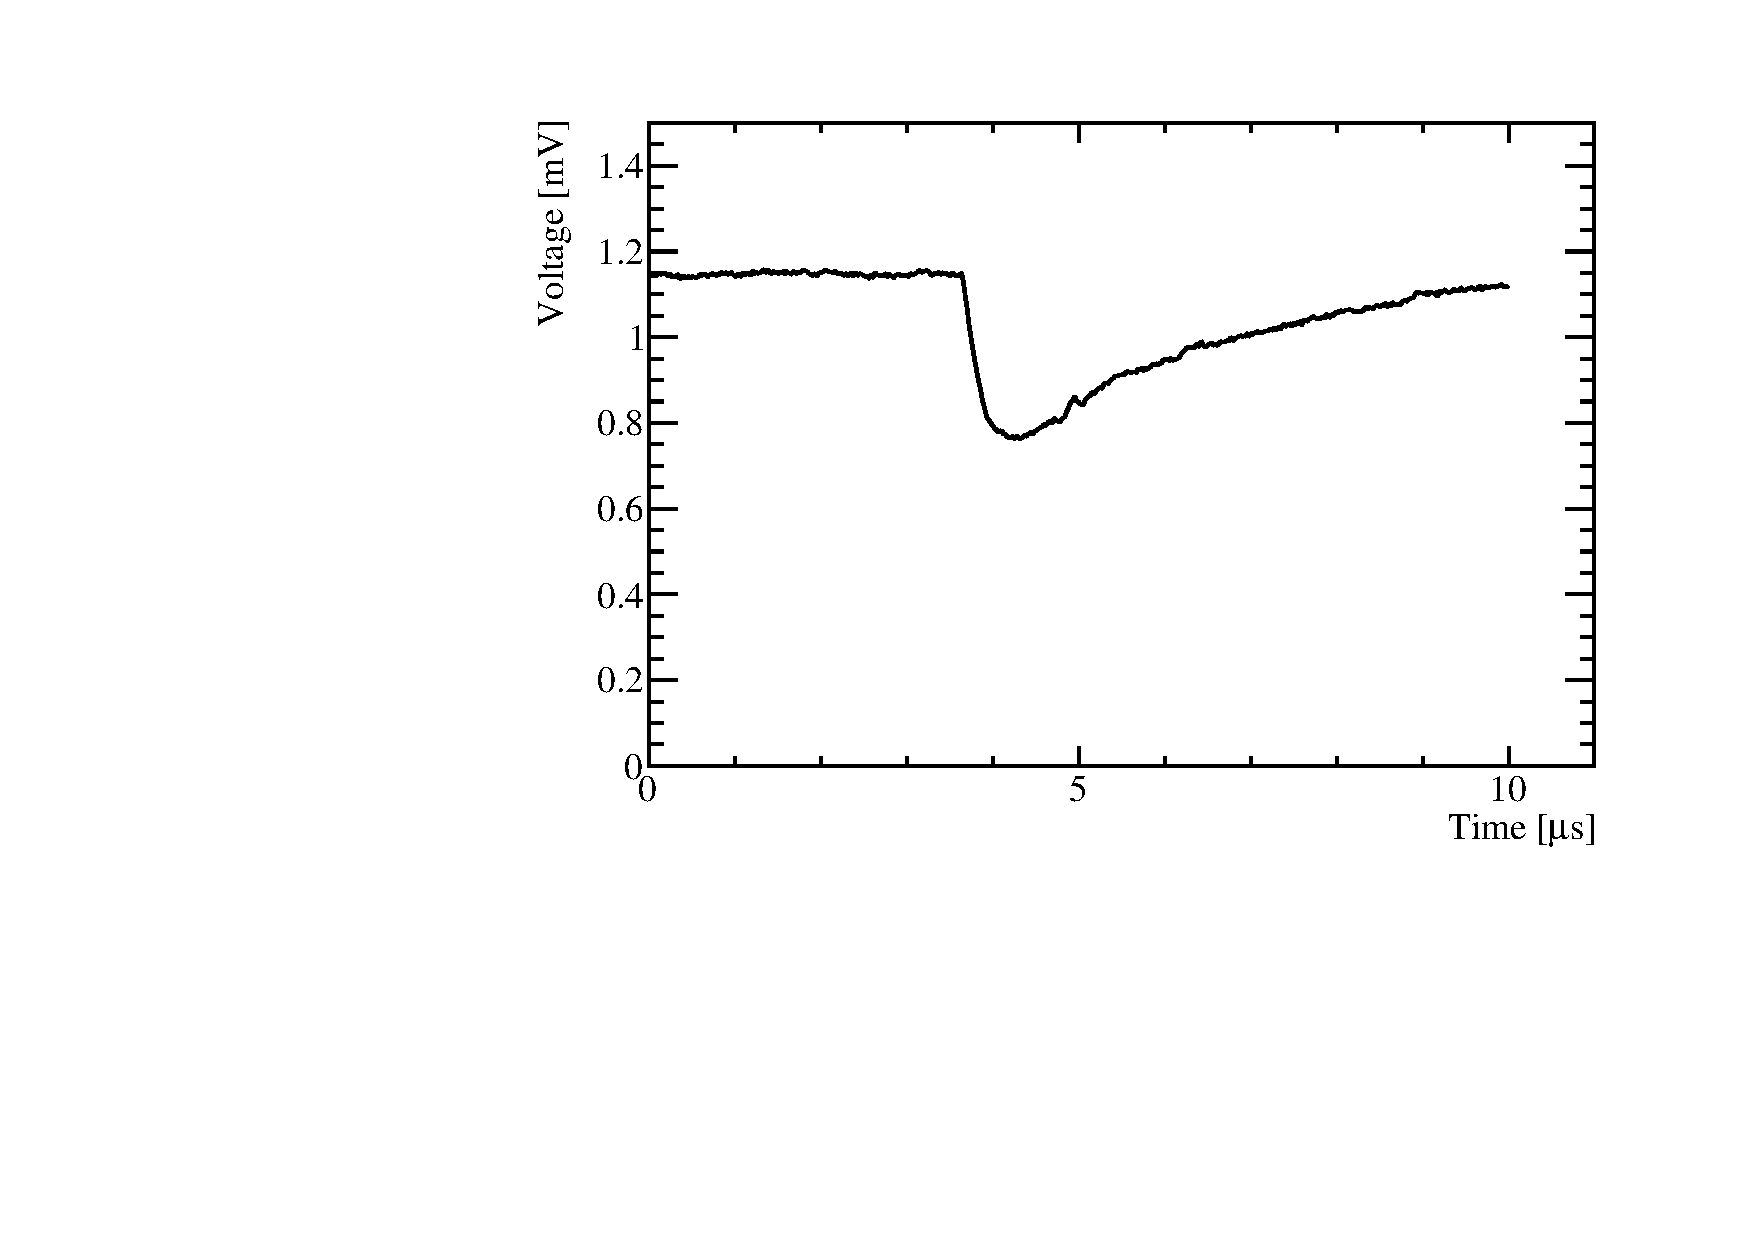
\includegraphics[width=0.5\textwidth]{CLICdpVertex/Plots/HV-CMOS/Frames/PulseShape01006NoOffset.pdf}}
\subfloat[]{\label{fig:pulseshape4}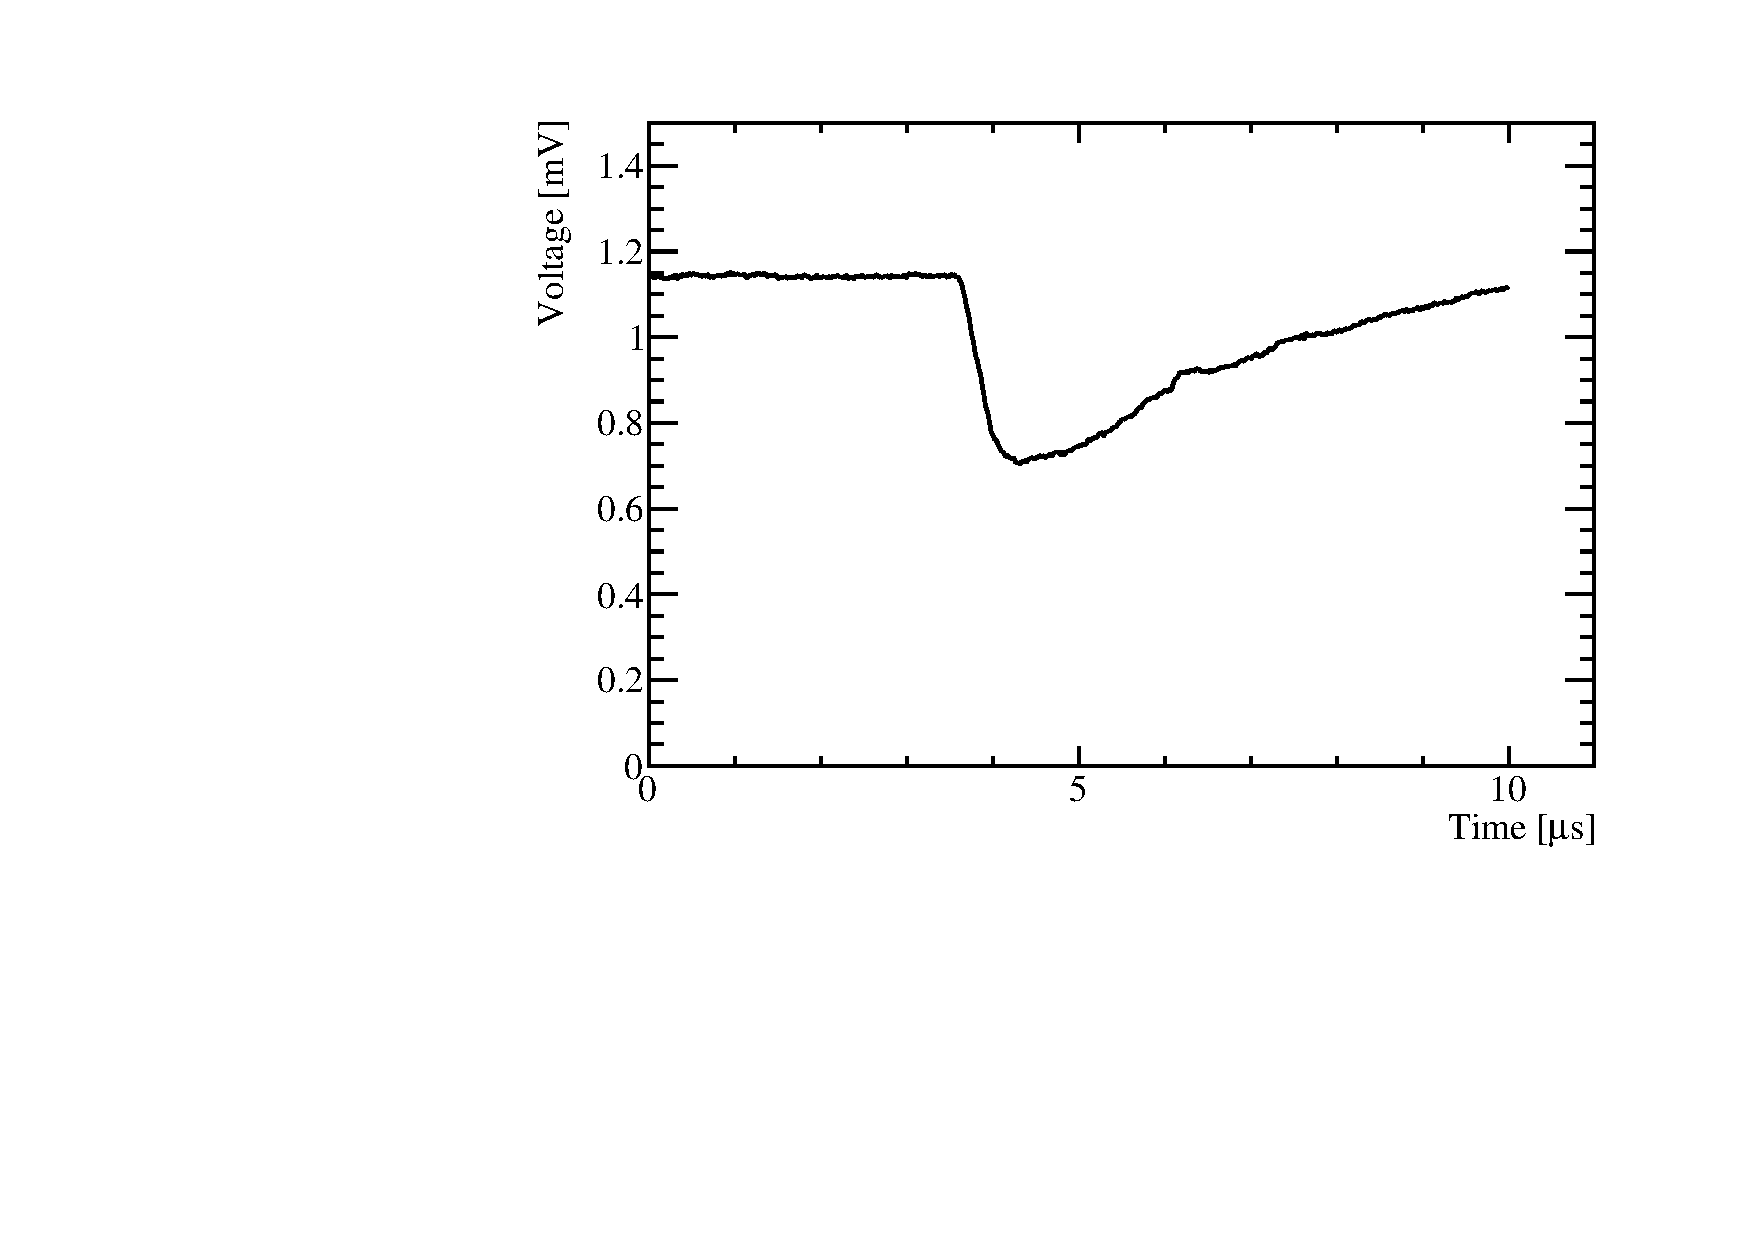
\includegraphics[width=0.5\textwidth]{CLICdpVertex/Plots/HV-CMOS/Frames/PulseShape01008NoOffset.pdf}}
\caption[CCPDv3 voltage pulses produced using a radioactive source, $\text{Sr}^{90}$, to deposit charge in the sensor.]{CCPDv3 voltage pulses produced using a radioactive source, $\text{Sr}^{90}$, to deposit charge in the sensor.}
\label{fig:pulseshapes}
\end{figure}

%========================================================================================

\subsubsection{Analysis}
The quantities of interest related to the CCPDv3 output voltage are the pulse height, defined as the peak of the voltage pulse, and the rise time, defined as the time it takes for the CCPDv3 to reach the pulse height.  For ease of analysis the baseline voltage is subtracted from the CCPDv3 output voltage and the pulse shape inverted before the following analysis is applied to extract the variables of interest.  

The pulse height is defined using a Gaussian fit to the peak of the voltage pulse.  This method is used to minimise the dependency of the pulse height on small fluctuations in the output voltage.  The peak of the voltage pulse is defined as the region where the change in the CCPDv3 voltage output is greater than 90\% of the maximum change in the CCPDv3 voltage output.  

The rise time is defined as the time taken for the signal to go from 10\% to 90\% of the maximum change in the CCPDv3 voltage output.  This definition makes the rise time metric more robust against fluctuations in the CCPDv3 voltage output.  

Examples of the calculation of these metrics for a representative pulse is shown in figure \ref{fig:pulseshapeanalysis}.  Due to the design of the CCPDv3 matrix, it is only possible to record the CCPDv3 voltage output for 15 pixels running along one edge of the 64 $\times$ 64 matrix.  Therefore, in the subsequent analysis, data was taken for each of these accessible pixels and combined.

\begin{figure}[h!]
\centering
\subfloat[]{\label{fig:pulseshapeanalysisvoltage}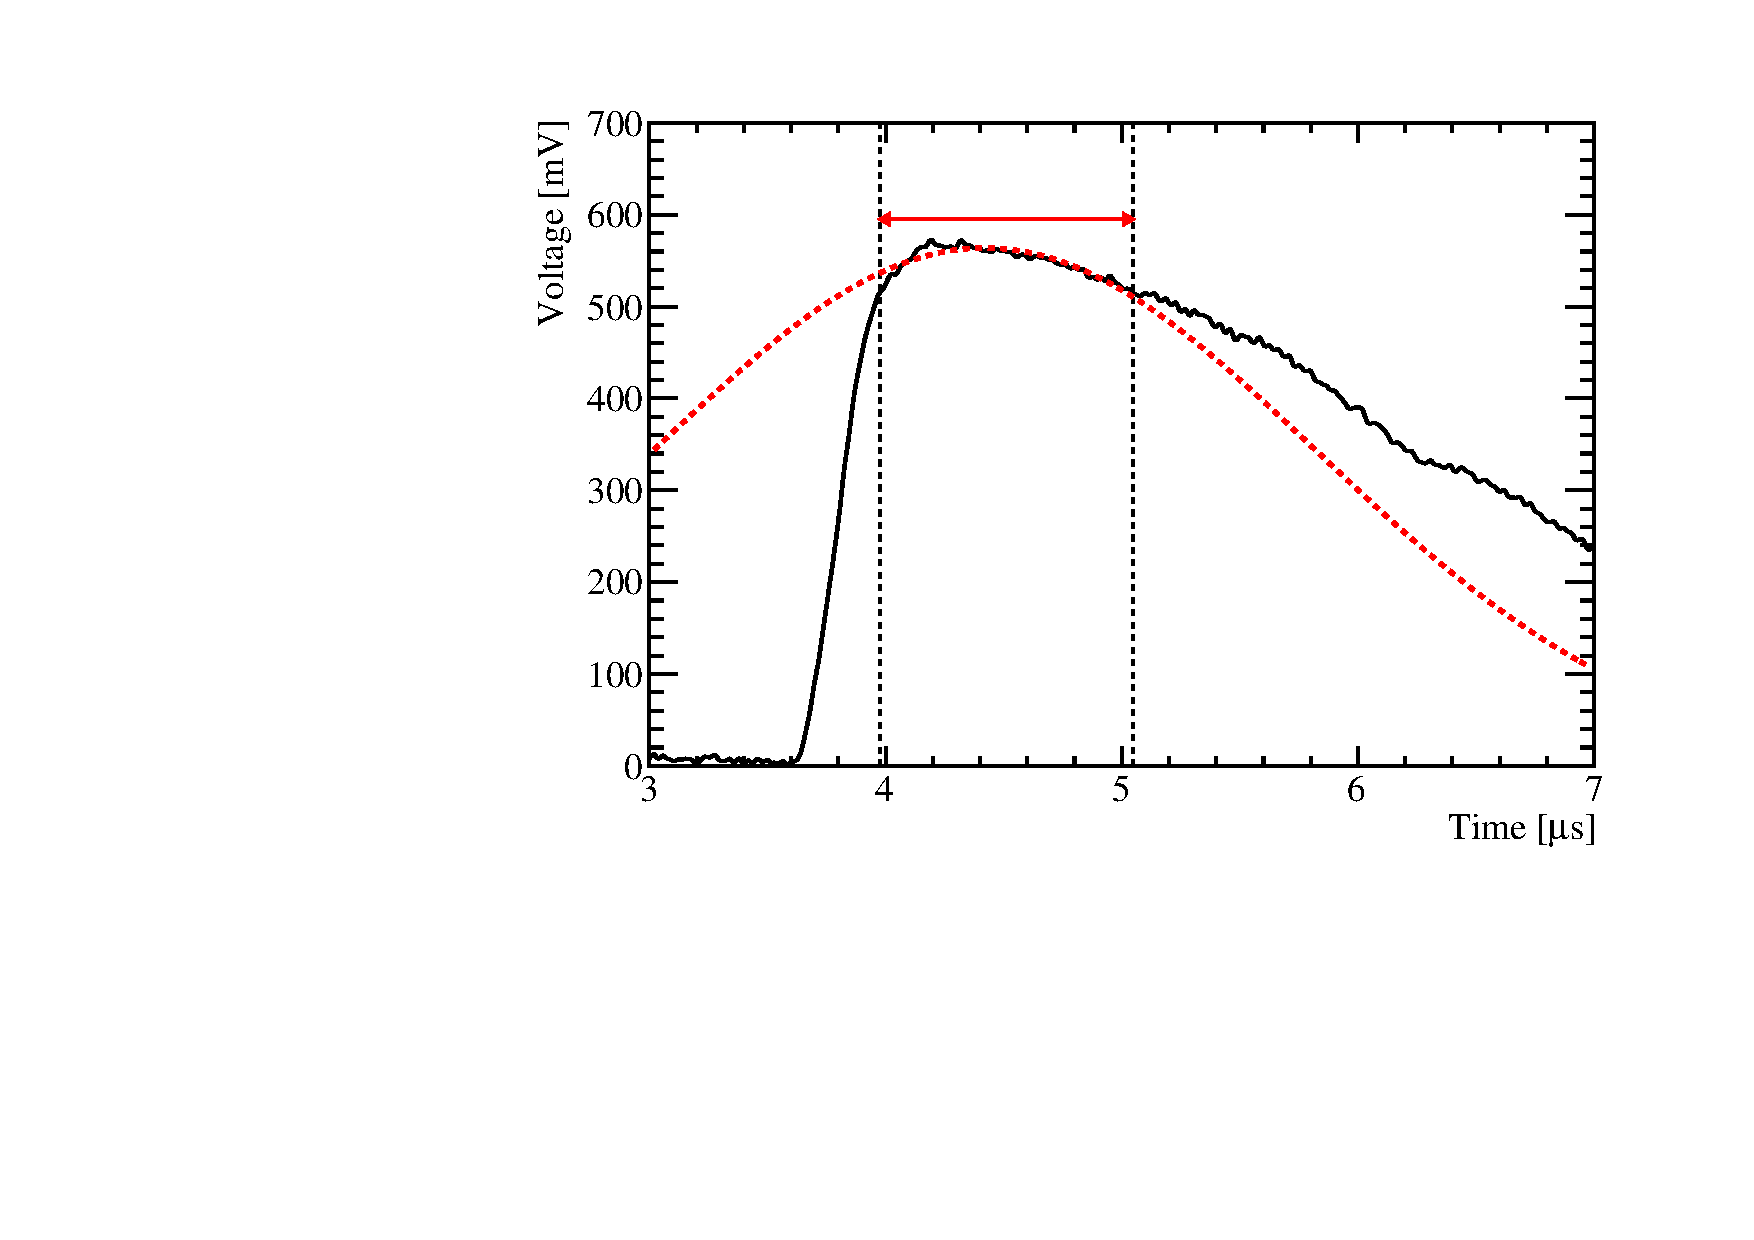
\includegraphics[width=0.5\textwidth]{CLICdpVertex/Plots/HV-CMOS/Frames/PulseShape01000FittingVoltage.pdf}}
\subfloat[]{\label{fig:pulseshapeanalysistime}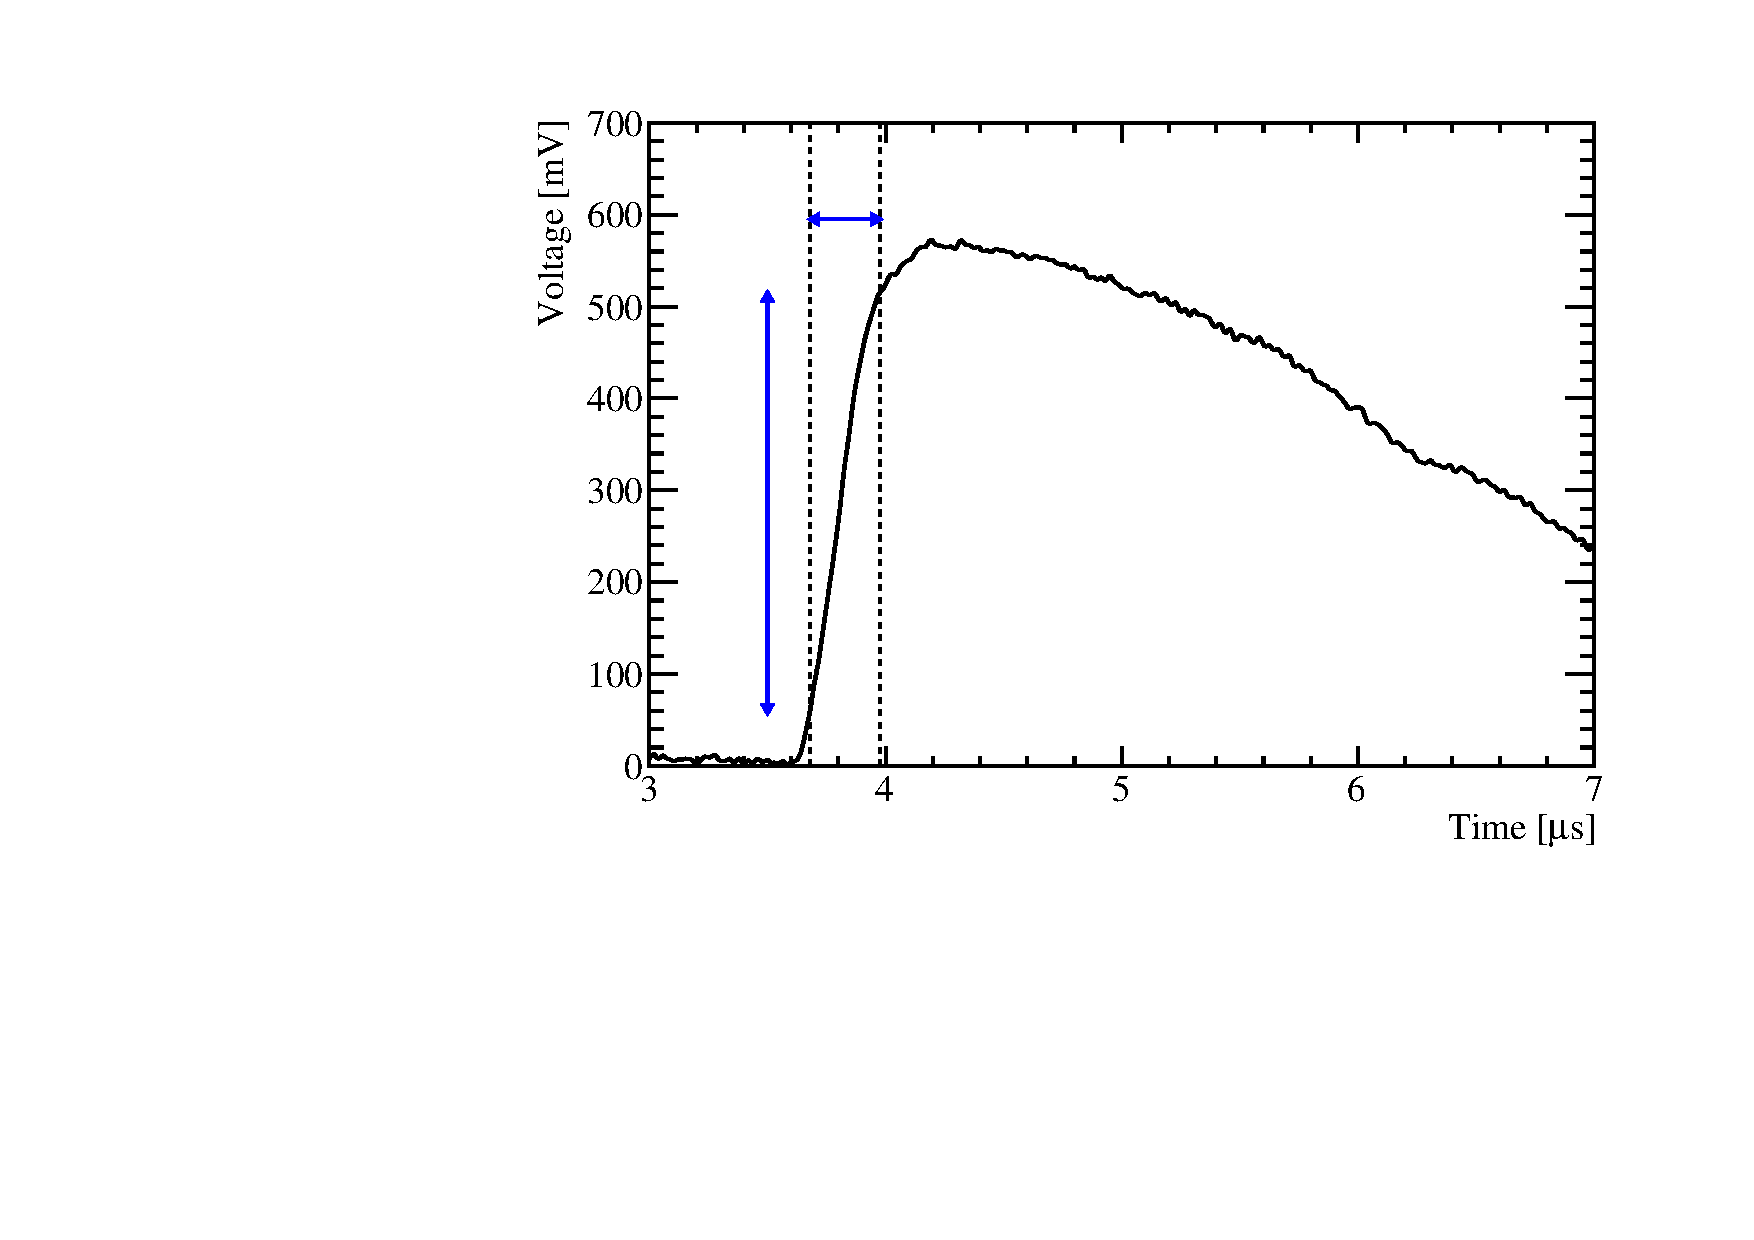
\includegraphics[width=0.5\textwidth]{CLICdpVertex/Plots/HV-CMOS/Frames/PulseShape01000FittingRiseTime.pdf}}
\caption[An example calculation of the pulse height and rise time for the CCPDv3 output voltage.  In this example the black line show the CCPDv3 output voltage as a function of time where the baseline voltage has been subtracted and the pulse shape inverted.  These voltage pulses were created using a radioactive source, $\text{Sr}^{90}$, to deposit charge in the sensor. \protect\subref{fig:pulseshapeanalysisvoltage} The definition of the pulse height.  Pulse height is defined as the amplitude of a Gaussian function fitted across the peak of the voltage pulse.  The peak of the voltage pulse is defined as the region where the voltage in excess of 90\% of the raw pulse height, which is indicated in the figure by the red arrow.  The red dotted line shows the Gaussian fit used to extract the pulse height.  \protect\subref{fig:pulseshapeanalysistime} The definition of rise time.  Rise time is defined as the time taken for the CCPDv3 voltage to rise from 10\% to 90\% of the raw pulse height.  The rise time, and change in CCPDv3 output voltage over this time, are shown in the figure by the blue arrows.]{An example calculation of the pulse height and rise time for the CCPDv3 output voltage.  In this example the black line show the CCPDv3 output voltage as a function of time where the baseline voltage has been subtracted and the pulse shape inverted.  These voltage pulses were created using a radioactive source, $\text{Sr}^{90}$, to deposit charge in the sensor. \protect\subref{fig:pulseshapeanalysisvoltage} The definition of the pulse height.  Pulse height is defined as the amplitude of a Gaussian function fitted across the peak of the voltage pulse.  The peak of the voltage pulse is defined as the region where the voltage in excess of 90\% of the raw pulse height, which is indicated in the figure by the red arrow.  The red dotted line shows the Gaussian fit used to extract the pulse height.  \protect\subref{fig:pulseshapeanalysistime} The definition of rise time.  Rise time is defined as the time taken for the CCPDv3 voltage to rise from 10\% to 90\% of the raw pulse height.  The rise time, and change in CCPDv3 output voltage over this time, are shown in the figure by the blue arrows.}
\label{fig:pulseshapeanalysis}
\end{figure}

%========================================================================================

\subsubsection{Results: Rise Time vs Pulse Height}
\label{sec:resultsrisetimepulseheight}
The mean rise time as function of pulse height for the CCPDv3 output voltage is shown in figure \ref{fig:risetime}.  This was determined by binning the measurements in pulse height and determining the mean rise time for measurements in each bin.  The pulse height was binned using a bin width of 4 mV ranging from 0 to 700 mV.  A minimum of 10 measurements per bin were used for the calculation of the average rise time.  The error bars on this figure show the standard error in the mean rise time.  Data was only included in this analysis if the on-pixel event counter registered a single hit in the time window used to take data.

\begin{figure}[h!]
\centering
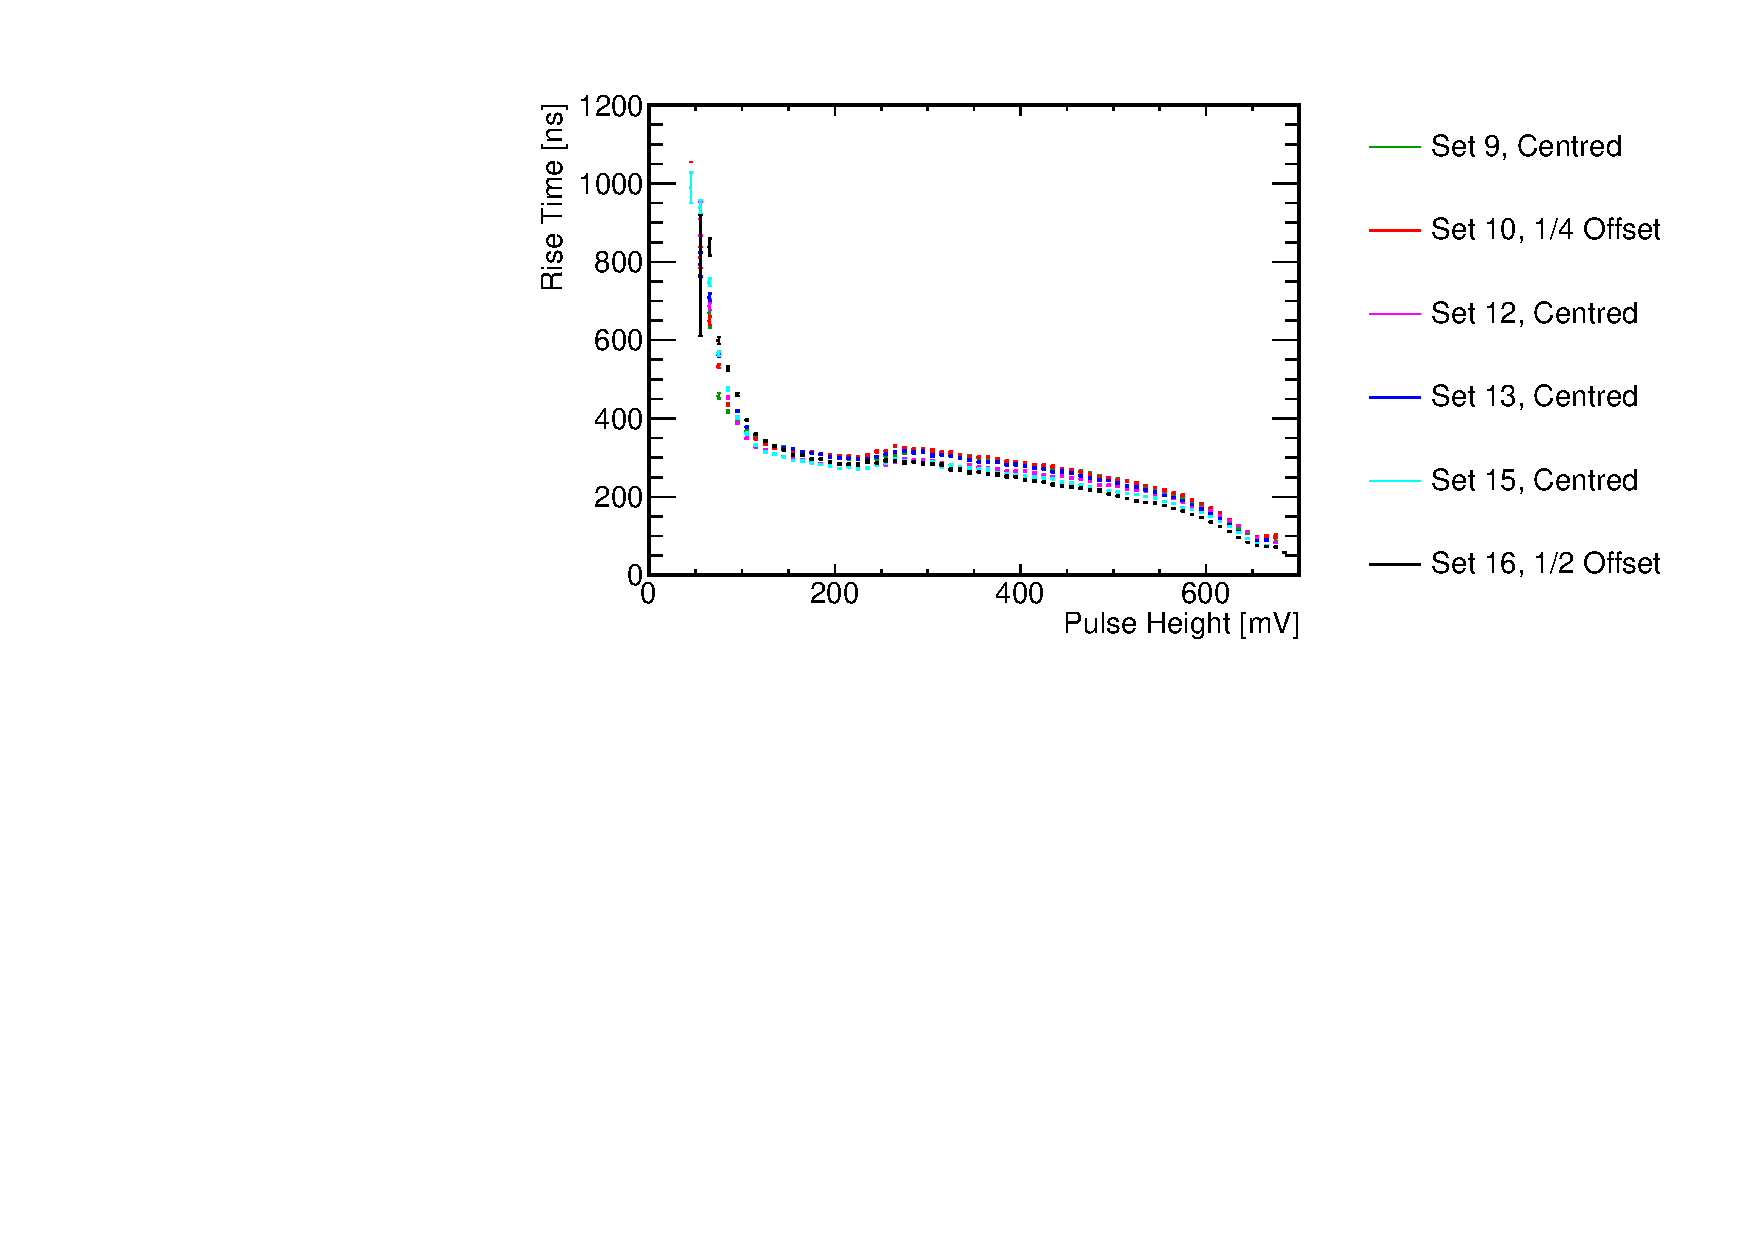
\includegraphics[width=1.0\textwidth]{CLICdpVertex/Plots/RadSourceAnalysis/AllSETs_RiseTime_PulseHeight.pdf}
\caption[The CCPDv3 output voltage rise time as a function of pulse height.]{The CCPDv3 output voltage rise time as a function of pulse height.}
\label{fig:risetime}
\end{figure}
 
The data in figure \ref{fig:risetime} shows that the rise time for the CCPDv3 front-end is approximately 300~ns across all samples.  The rise time is largely independent of pulse height for all but the smallest signals.  For very small pulse heights ($< 100$ mV) rise times are significantly larger, which suggests that the deposited charge takes a longer time to be collected.  This may be due to charge transport occurring via diffusion rather than drift.  A gradual reduction in the rise time is observed as the total deposited charge, which is proportional to the pulse height, increases.  This is expected as larger charge deposits in the sensor bulk lead to a greater rate of charge collection by the CCPDv3 and a smaller time taken for the pulse height to reach the peak.  As the intrinsic performance of the CCPDv3 sensors in the devices tested is very similar, comparisons of the misaligned samples will be made more straightforward.  As nearly identical intrinsic performance was observed for the CLICpix readout chips, as will be shown in section \ref{sec:testpulsecalibration}, any performance differences observed between these devices will be entirely due to the capacitive glue layer and the pad alignment.    

%========================================================================================

\subsubsection{Results: ToT vs Pulse Height}
\label{sec:resultstotpulseheight}
The mean ToT measured in the CLICpix as a function of the CCPDv3 output voltage pulse height is shown in figure \ref{fig:tot}.  Determination of the mean and error bars for the ToT as a function of pulse height measurement is identical to that described in section \ref{sec:resultsrisetimepulseheight} for the rise time as a function of pulse height measurement.   

\begin{figure}[h!]
\centering
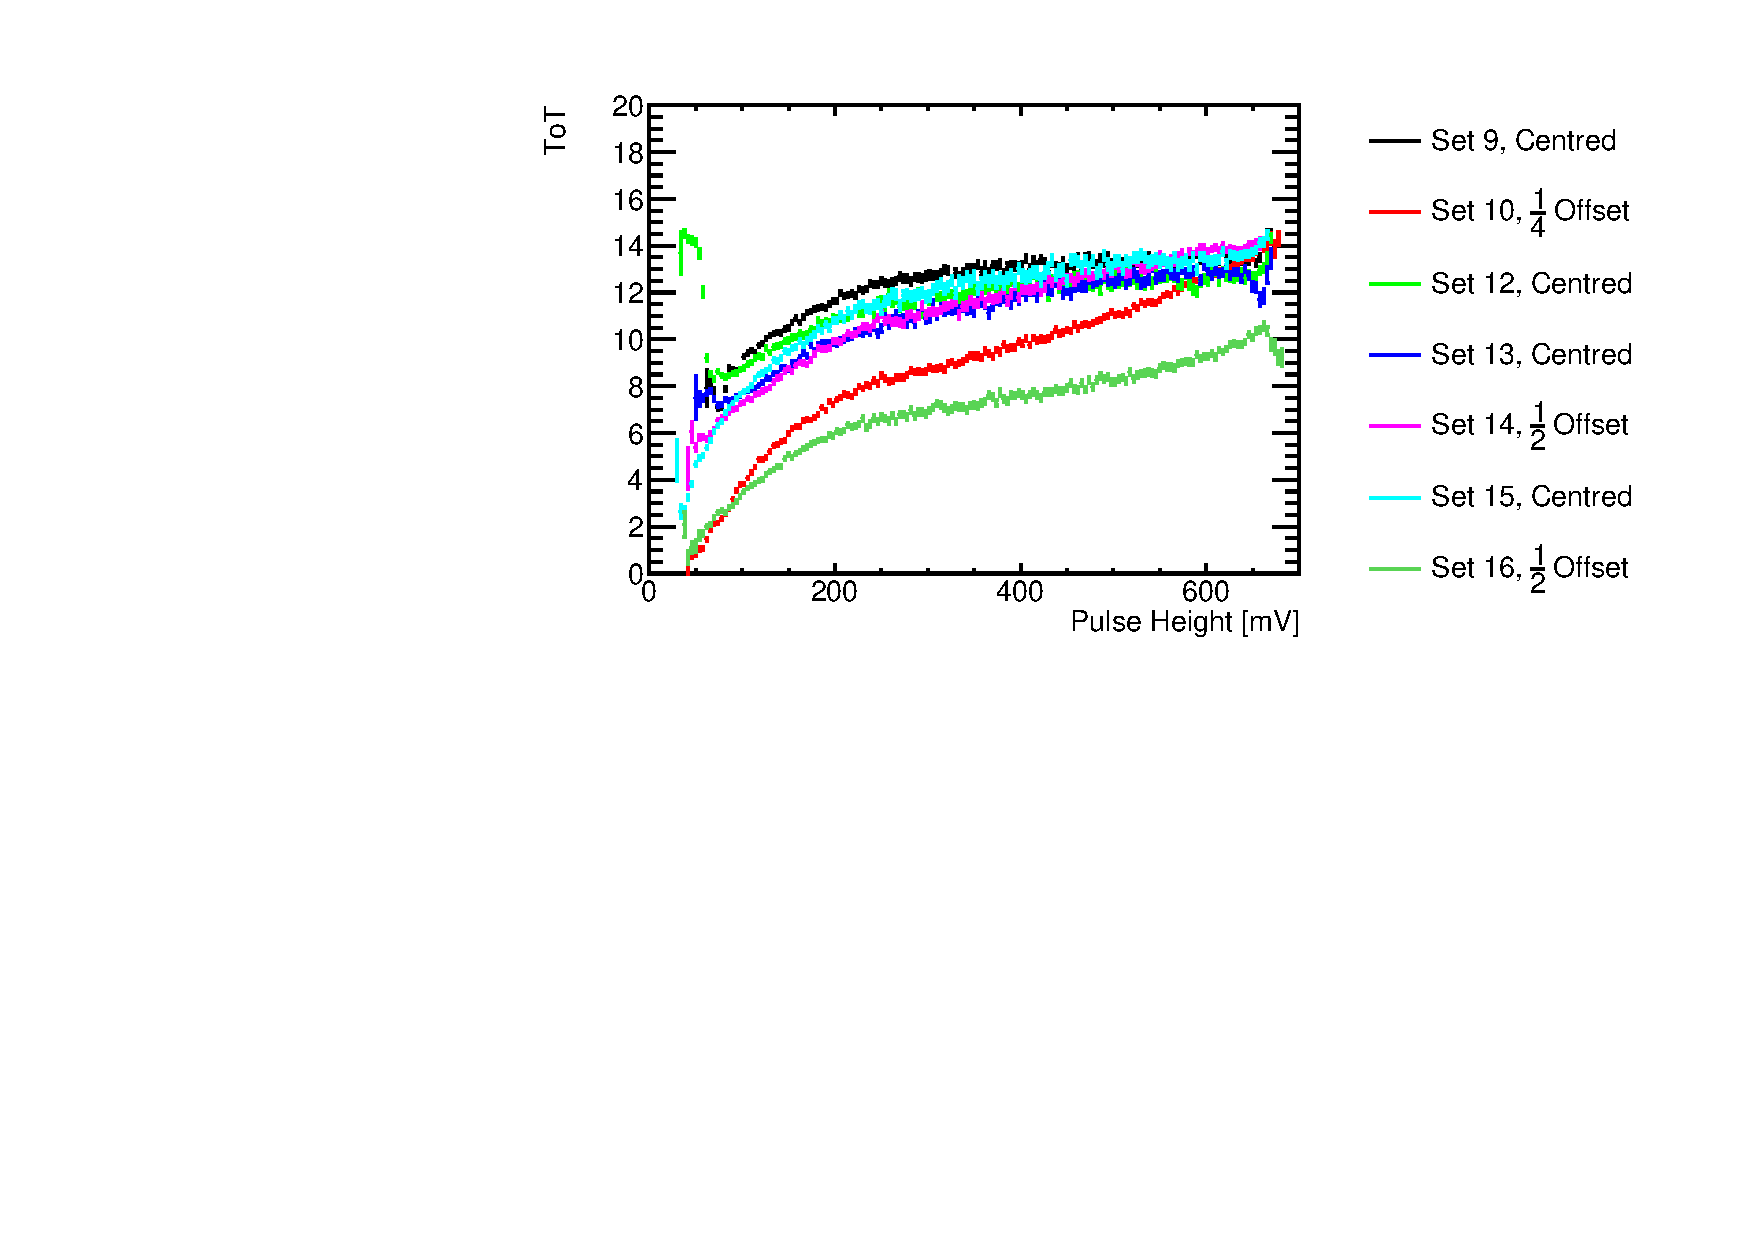
\includegraphics[width=1.0\textwidth]{CLICdpVertex/Plots/RadSourceAnalysis/AllSETs_TargetTot_PulseHeight.pdf}
\caption[The mean ToT measured on the CLICpix ASIC as a function of CCPDv3 voltage pulse height.]{The mean ToT measured on the CLICpix ASIC as a function of CCPDv3 voltage pulse height.}
\label{fig:tot}
\end{figure}

For samples where the CCPDv3 and CLICpix are centred, the distribution of the mean ToT against pulse height shows that the ToT increases with pulse height up to values of approximately 400~mV and for larger pulse heights the mean ToT saturates at $\approx 15$.  It is expected that the $\frac{1}{4}-$ and $\frac{1}{2}-$offset samples will have a lower ToT than the centred samples due to the lower effective capacitance between the CCPDv3 and CLICpix pads.  The greater the offset, the smaller the effective capacitance to the target CLICpix pad will be, and so the lower the recorded ToT.  This is can be seen when comparing the centred samples to SET 10, the $\frac{1}{4}-$offset sample, and SET 16, the $\frac{1}{2}-$offset sample.  In addition to the charge injected by the radioactive source there will also be background noise present from a variety of effects such as manufacturing defects in the silicon and thermal noise.  This additional charge will increase the mean ToT recorded by the CLICpix and is the most likely reason as to why the mean ToT does not smoothly tend to zero as the pulse height decreases.

%========================================================================================

\subsubsection{Results: Cross Couplings}
Capacitive coupling of the sensor to the readout ASIC can also lead to unwanted signals being induced on neighbouring pixels, due to non-zero stray capacitances. Cross-coupling is the transfer of signal from a sensor pad to the readout ASIC on an adjacent pad, which will occur if there is a non-negligible capacitance between the two pads.  Signals are still transferred between the aligned sensor and readout pads, however, if the cross-capacitance is large enough unwanted additional hits in the neighbouring pads will be created.  This issue is particularly relevant for this study as any misalignment between the sensor and readout pads will result in an increase in the cross-capacitance along the direction of the misalignment.   

Any effects of cross-coupling can be studied using the same setup as was used in section \ref{sec:resultstotpulseheight} for the ToT against pulse height analysis, but in contrast considering the ToT on the adjacent CLICpix pixel along the direction of the misalignment.  The mean ToT on the adjacent pixel is shown as a function of the pulse height for all devices where the CCPDv3 and CLICpix are aligned in figure \ref{fig:totcrosscoupling1} and for the misaligned samples in figure \ref{fig:totcrosscoupling2}.

\begin{figure}[h!]
\centering
\subfloat[]{\label{fig:totcrosscoupling1}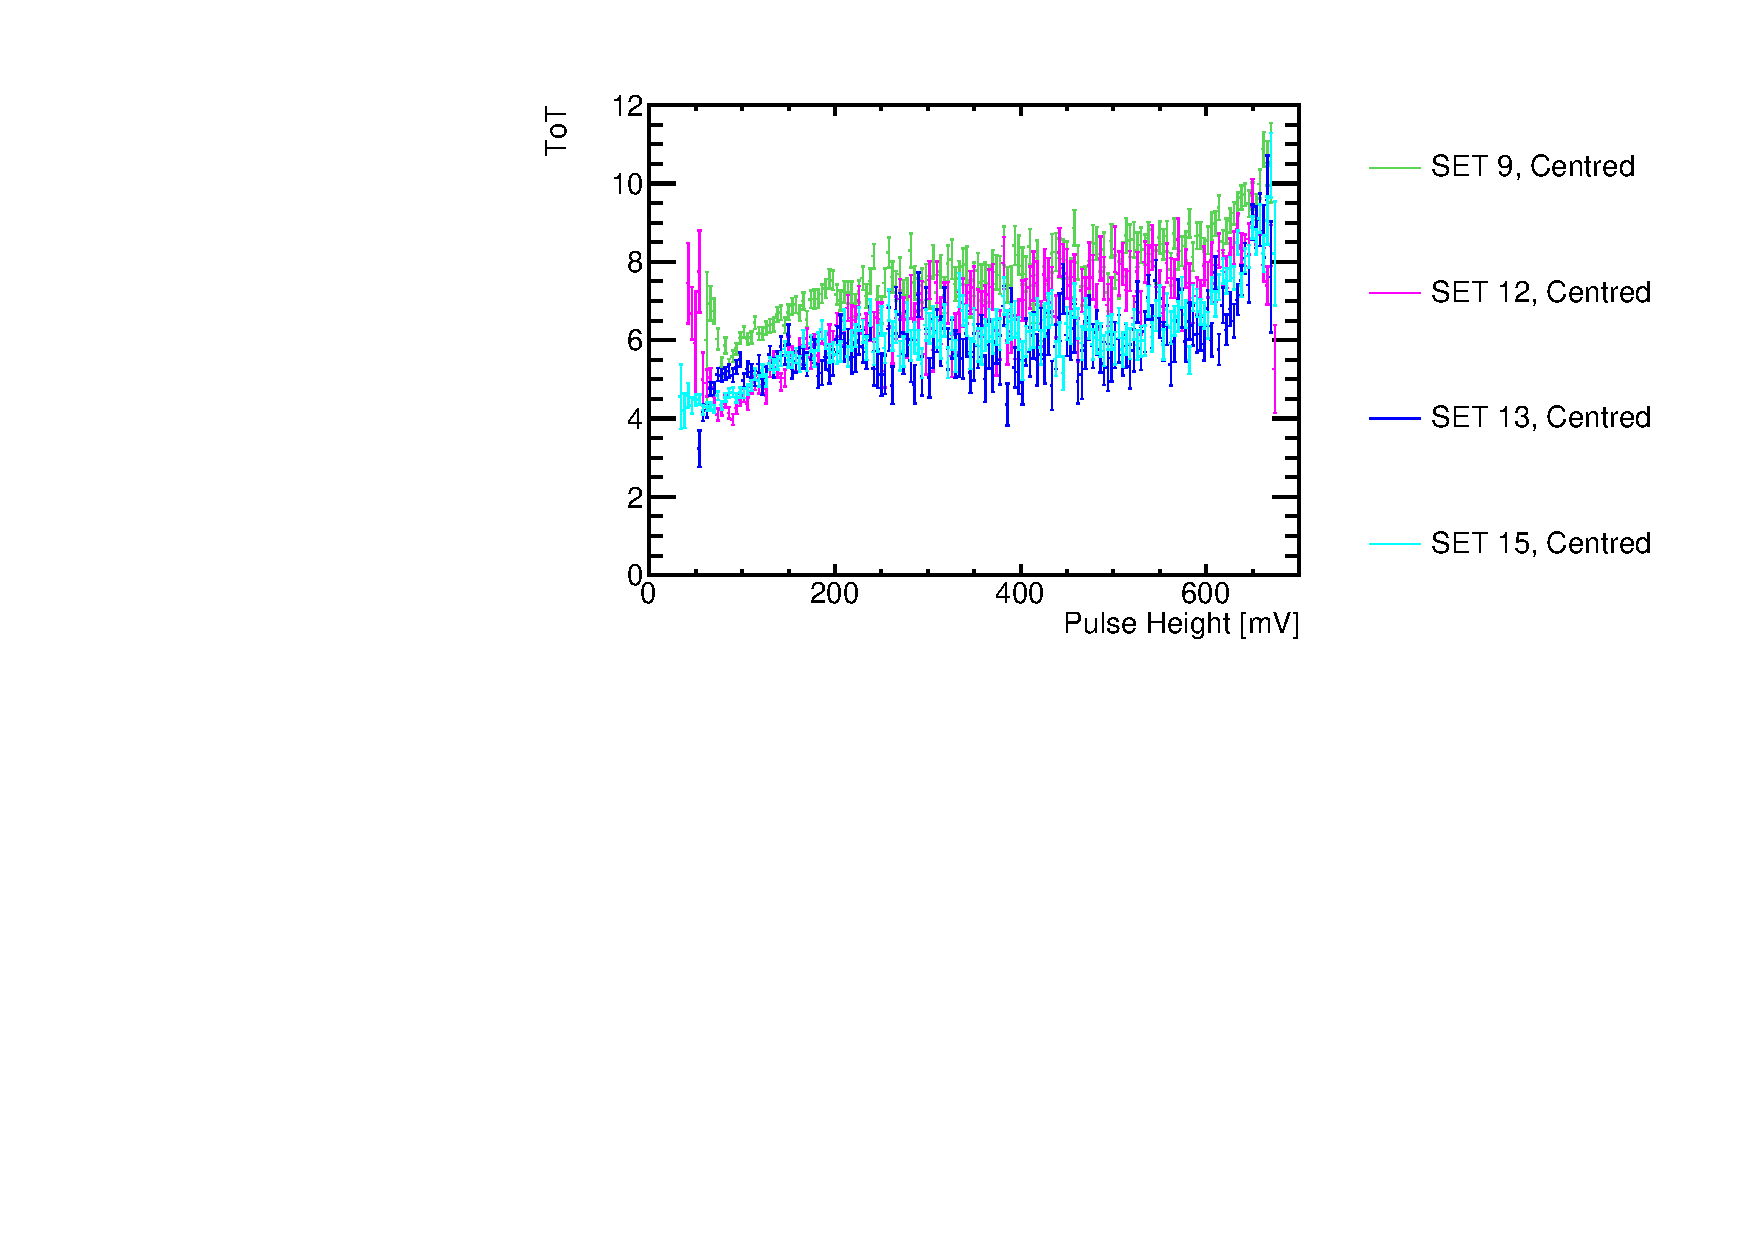
\includegraphics[width=1.0\textwidth]{CLICdpVertex/Plots/RadSourceAnalysis/NoCrossCouplingSETs_Tot_X_PulseHeight.pdf}}\hfill
\subfloat[]{\label{fig:totcrosscoupling2}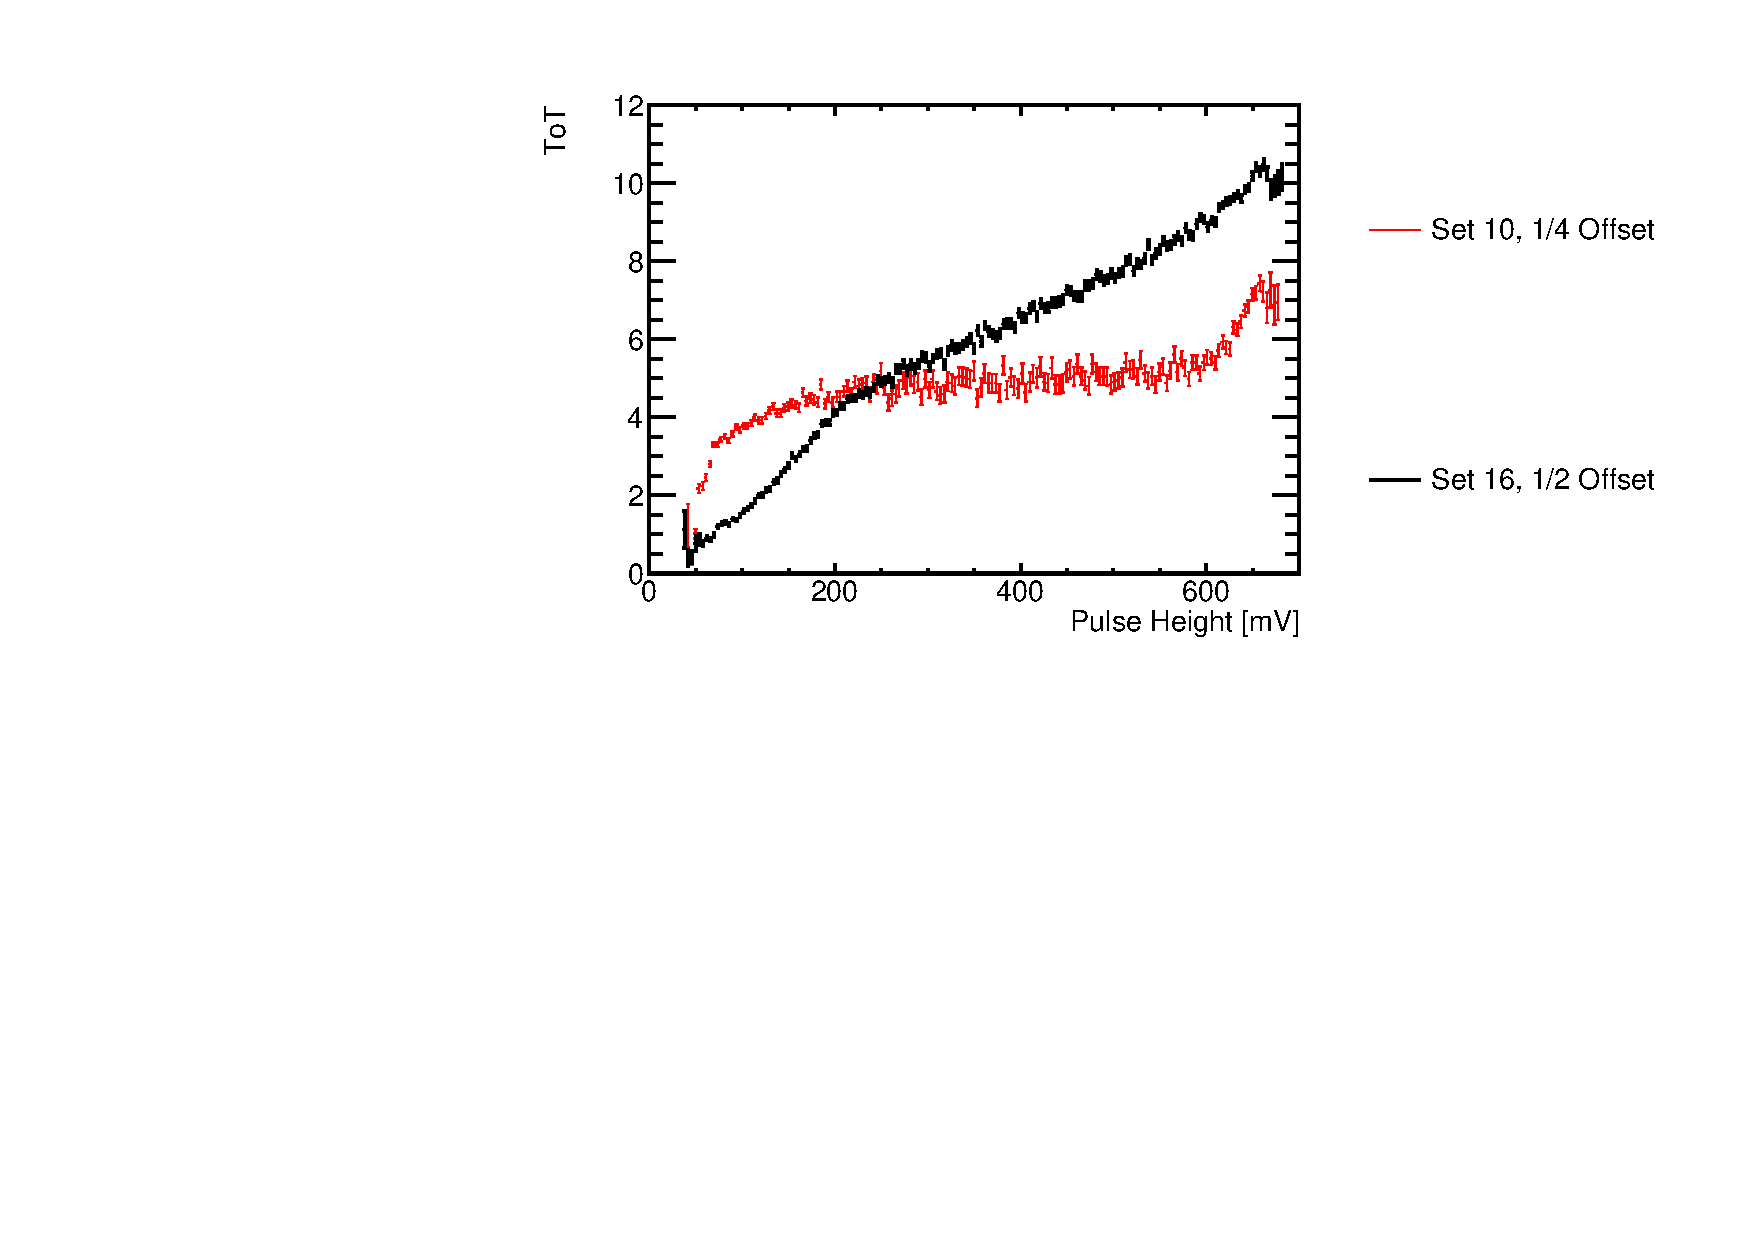
\includegraphics[width=1.0\textwidth]{CLICdpVertex/Plots/RadSourceAnalysis/CrossCouplingSETs_Tot_X_PulseHeight.pdf}}
\caption[The mean ToT measured on the adjacent CLICpix pixel, along the direction of the offset, as a function of CCPDv3 voltage pulse height for \protect\subref{fig:totcrosscoupling1} the centred and \protect\subref{fig:totcrosscoupling2} the misaligned devices.]{The mean ToT measured on the adjacent CLICpix pixel, along the direction of the offset, as a function of CCPDv3 voltage pulse height for \protect\subref{fig:totcrosscoupling1} the centred and \protect\subref{fig:totcrosscoupling2} the misaligned devices.}
\label{fig:totcrosscoupling}
\end{figure}

The distributions of the mean ToT on the adjacent CLICpix as a function of pulse height are governed largely by cross-coupling effects.  These effects will make this distribution look similar in shape to that of the mean ToT in the target CLICpix as a function of pulse height, shown in figure \ref{fig:tot}.  However, the gradient of the adjacent ToT distribution will be shallower than the adjacent ToT distribution as the cross-capacitance is smaller than the aligned capacitance.  The exception to this is the $\frac{1}{2}-$offset sample where the cross-capacitance and aligned capacitance will be comparable.  In addition to cross-coupling, this distribution will be affected by electrical noise and charge being deposited in the neighbouring HV-CMOS pixels.  

For the centred samples, cross-coupling seems to have a small effect as the correlation between the adjacent ToT and pulse height is minimal.  For the $\frac{1}{4}-$offset sample there is a stronger correlation between the adjacent ToT and pulse height, which indicates that cross-coupling is having a more dominant effect.  The gradient of the adjacent ToT vs pulse height is, however, very shallow as the cross-capacitance for this device will be relatively small.  A much stronger cross-capacitive effect can be see in the $\frac{1}{2}-$offset sample, which is expected given it has a larger cross-capacitance than either the centred or $\frac{1}{4}-$offset sample.  The adjacent ToT distribution for the $\frac{1}{2}-$offset sample almost mirrors the aligned ToT distribution in terms of both shape and width of the distribution.  There are some small differences between the shape of the aligned and adjacent ToT vs pulse height distribution for the $\frac{1}{2}-$offset sample, but this is understood to be from the column structure of the CLICpix readout ASIC, more details of which can be found in section \ref{sec:testpulsecalibration}.  Overall, these results indicate that, as expected, a misalignment between the CCPDv3 and CLICpix pads increases the effect of cross-coupling along the direction of the misalignment.

%========================================================================================

\subsection{Test Pulse Calibration}
\label{sec:testpulsecalibration}
In order to fully understand the charge transfer to the CLICpix, a calibration of the CLICpix front-end electronics response was performed.  This was achieved by directly injecting a voltage pulse of fixed height directly into a capacitor help in each CLICpix pixel.  This capacitor will then inject a known amount of charge into the pixel, and by varying the height of the pulse applied the response of the CLICpix to different amounts of charge can be quantified.  This experiment extends the characterisation of the CLICpix chip beyond what was found using the radioactive source measurements, as applying the voltage directly to the CLICpix fully isolates the response of the chip from any effects relating to the glue layer or CCPDv3.  

%========================================================================================

\subsubsection{Experimental Setup}

To prevent any influence from neighbouring pixels during the test pulse measurements the matrix was pulsed in stages.  Charge was injected into 1 out of every 16 pixels while masking the others to ensure issues related to power consumption were not encountered.  This was repeated 15 more times using different mask configurations until the entire matrix had been sampled.  This procedure was carried out 100 times to determine the average ToT response on a per-pixel level.  The pulse height injected into the CLICpix was varied from 2 to 180 mV in steps of 2 mV in order to fully characterise the response up to saturation of the ToT output.  An example of the mean ToT plotted against the injected pulse height is shown in figure \ref{fig:testpulseexamplenofit}.  

\begin{figure}[h!]
\centering
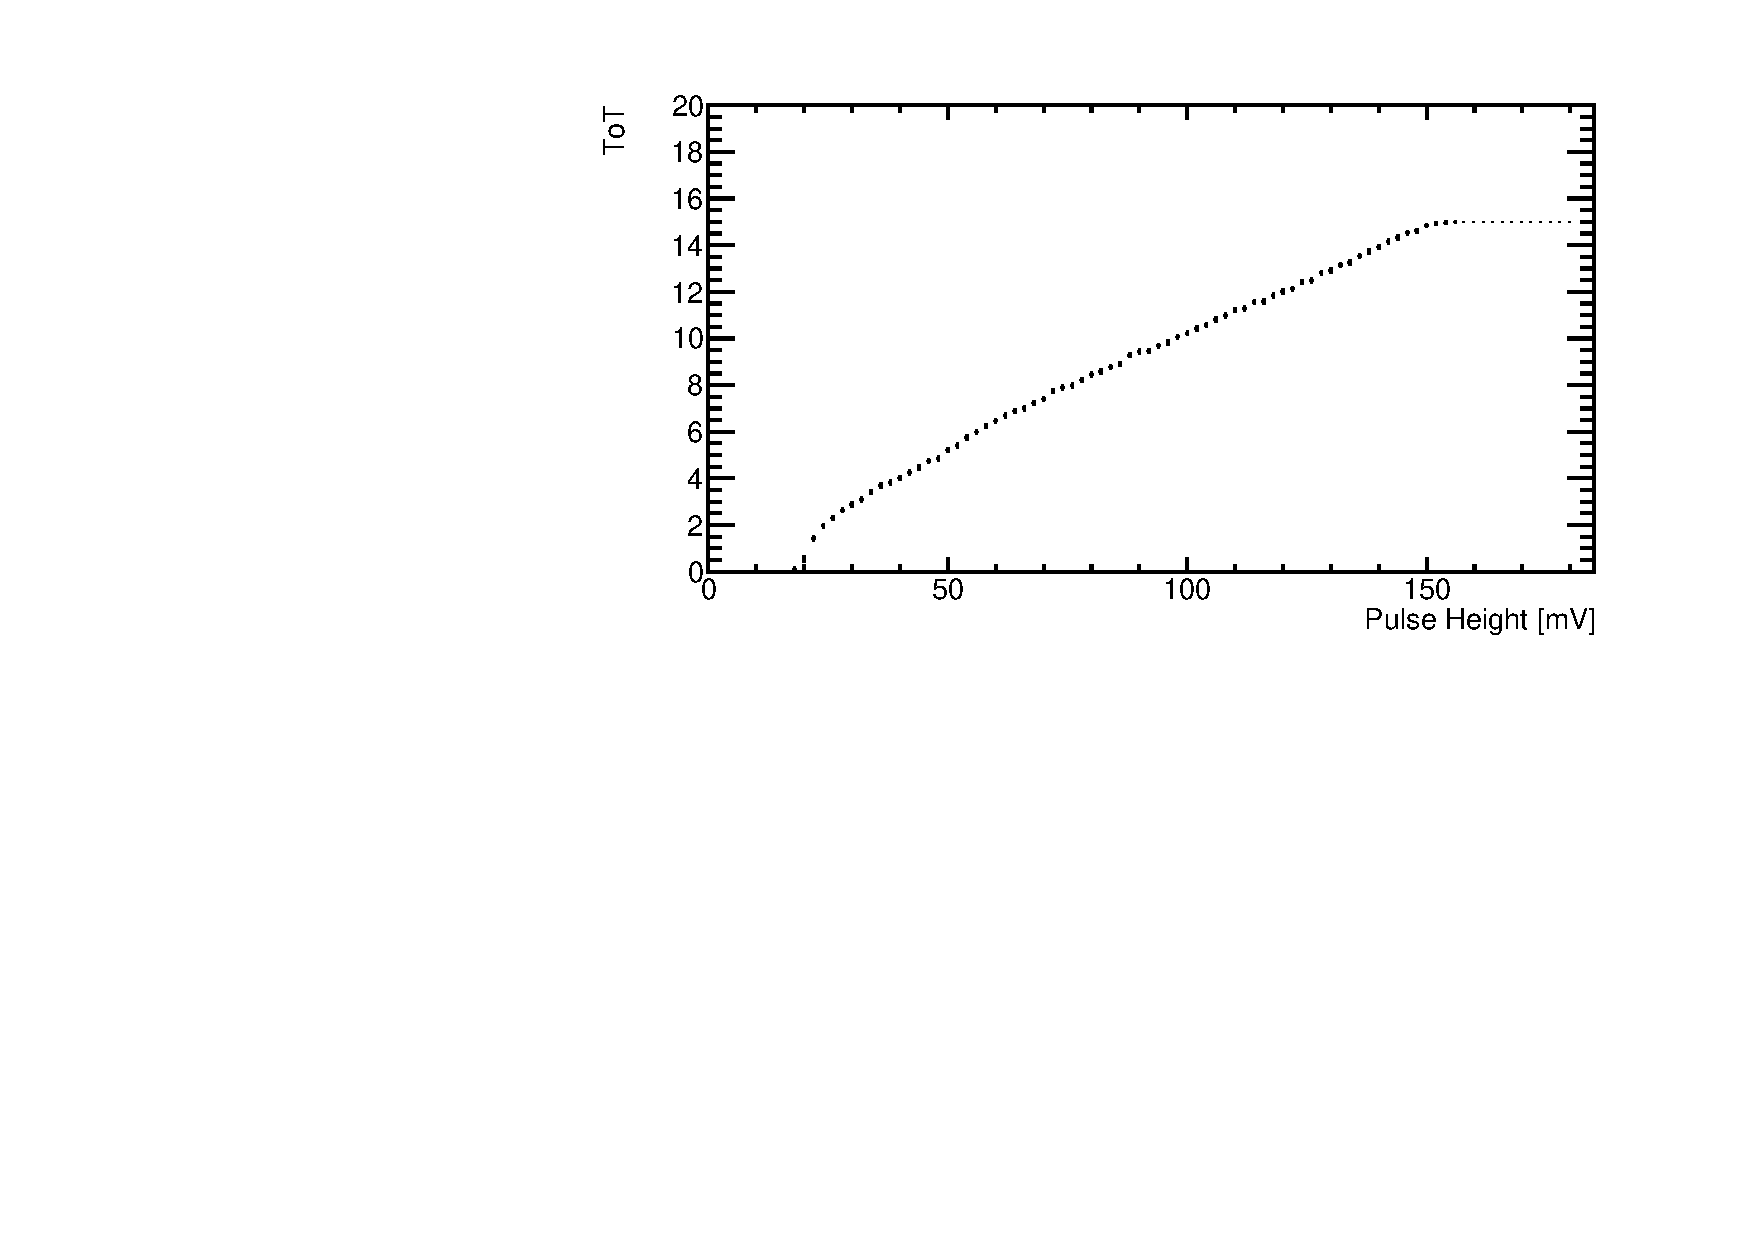
\includegraphics[width=1.0\textwidth]{CLICdpVertex/Plots/TestPulseCalibration/Fits/Set9/ToT_PulseHeight_Set_9_ChipID_001ec0db94b1_Pixel_x0_y0_NoFit.pdf}
\caption[The CLICpix ToT as a function of injected pulse height.  The black markers show the mean ToT and the error bars show the standard error.]{The CLICpix ToT as a function of injected pulse height.  The black markers show the mean ToT and the error bars show the standard error.}
\label{fig:testpulseexamplenofit}
\end{figure}

%========================================================================================

\subsubsection{Analysis}
The functional form of the ToT against pulse height plot will be described using a surrogate function \cite{AlipourTehrani:2054922}
\begin{equation}
y  = ax + b  - \frac{c}{x-t} \text{,}
\end{equation}

\noindent where $y$ is the ToT, $x$ is the pulse height in mV and $a$, $b$, $c$ and $t$ are fit parameters.  Application of the fit helps to condense the large amount of data recorded for an individual pixel down to a small number of parameters, which makes categorisation of the response of the CLICpix matrix clearer.  At large pulse heights the linear relationship dominates, while for low pulse heights the inversely proportional term dominates.  $c$ describes the curvature of the graph, while $t$ determines the asymptote below which no signal is detected.  Figure \ref{fig:testpulseexamplefit} shows an example of the application of this fit.  As this function does not describe saturation of the ToT or the region below threshold, the fit is only applied on data points where the mean ToT is greater than 1 and less than 14.75.  

\begin{figure}
\centering
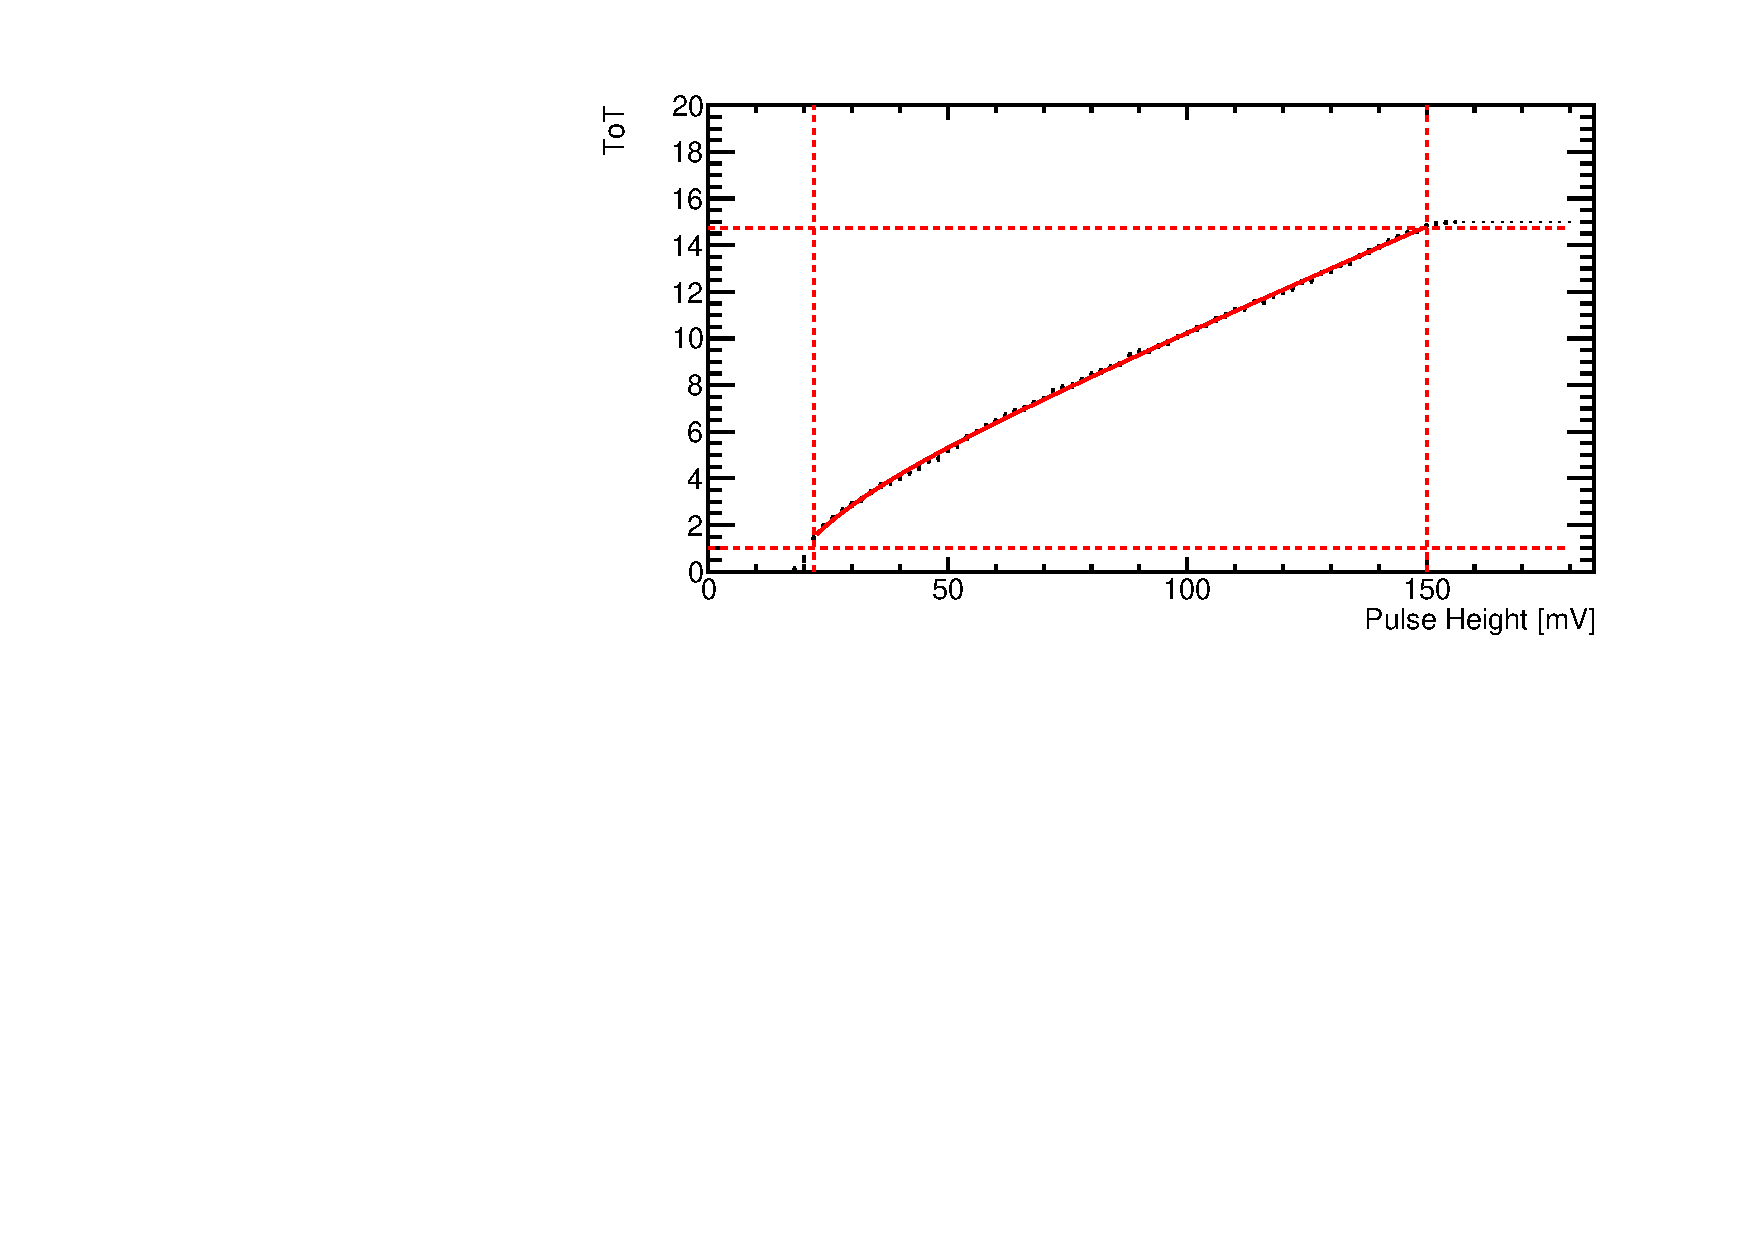
\includegraphics[width=1.0\textwidth]{CLICdpVertex/Plots/TestPulseCalibration/Fits/Set9/ToT_PulseHeight_Set_9_ChipID_001ec0db94b1_Pixel_x0_y0_Fit.pdf}
\caption[CLICpix ToT as a function of injected pulse height.]{CLICpix ToT as a function of injected pulse height for a single pixel.  The black markers are the mean ToT and the error bars are the standard error on the mean.  The solid red line shows the surrogate function fit and the dotted red lines show the range where the fit was applied.}
\label{fig:testpulseexamplefit}
\end{figure}

%========================================================================================

\subsubsection{Results}
\label{sec:testpulsecalibrationresults}
A known issue with the design of the CLICpix ASIC is the unwanted feedback capacitance between the discriminator output and amplifier input.  This feedback leads to an additional fixed injected charge being measured for each recorded hit, due to the firing of the discriminator.  The magnitude of this effect differs between even and odd columns across the CLICpix matrix due to slight differences in the physical layouts of alternating columns.  By examining the distribution of the surrogate fit parameters, shown for SET 9 in figure \ref{fig:fitparams}, this effect can be seen.  

\begin{figure}[h!]
\centering
\subfloat[$a$ parameter.]{\label{fig:fitparams1}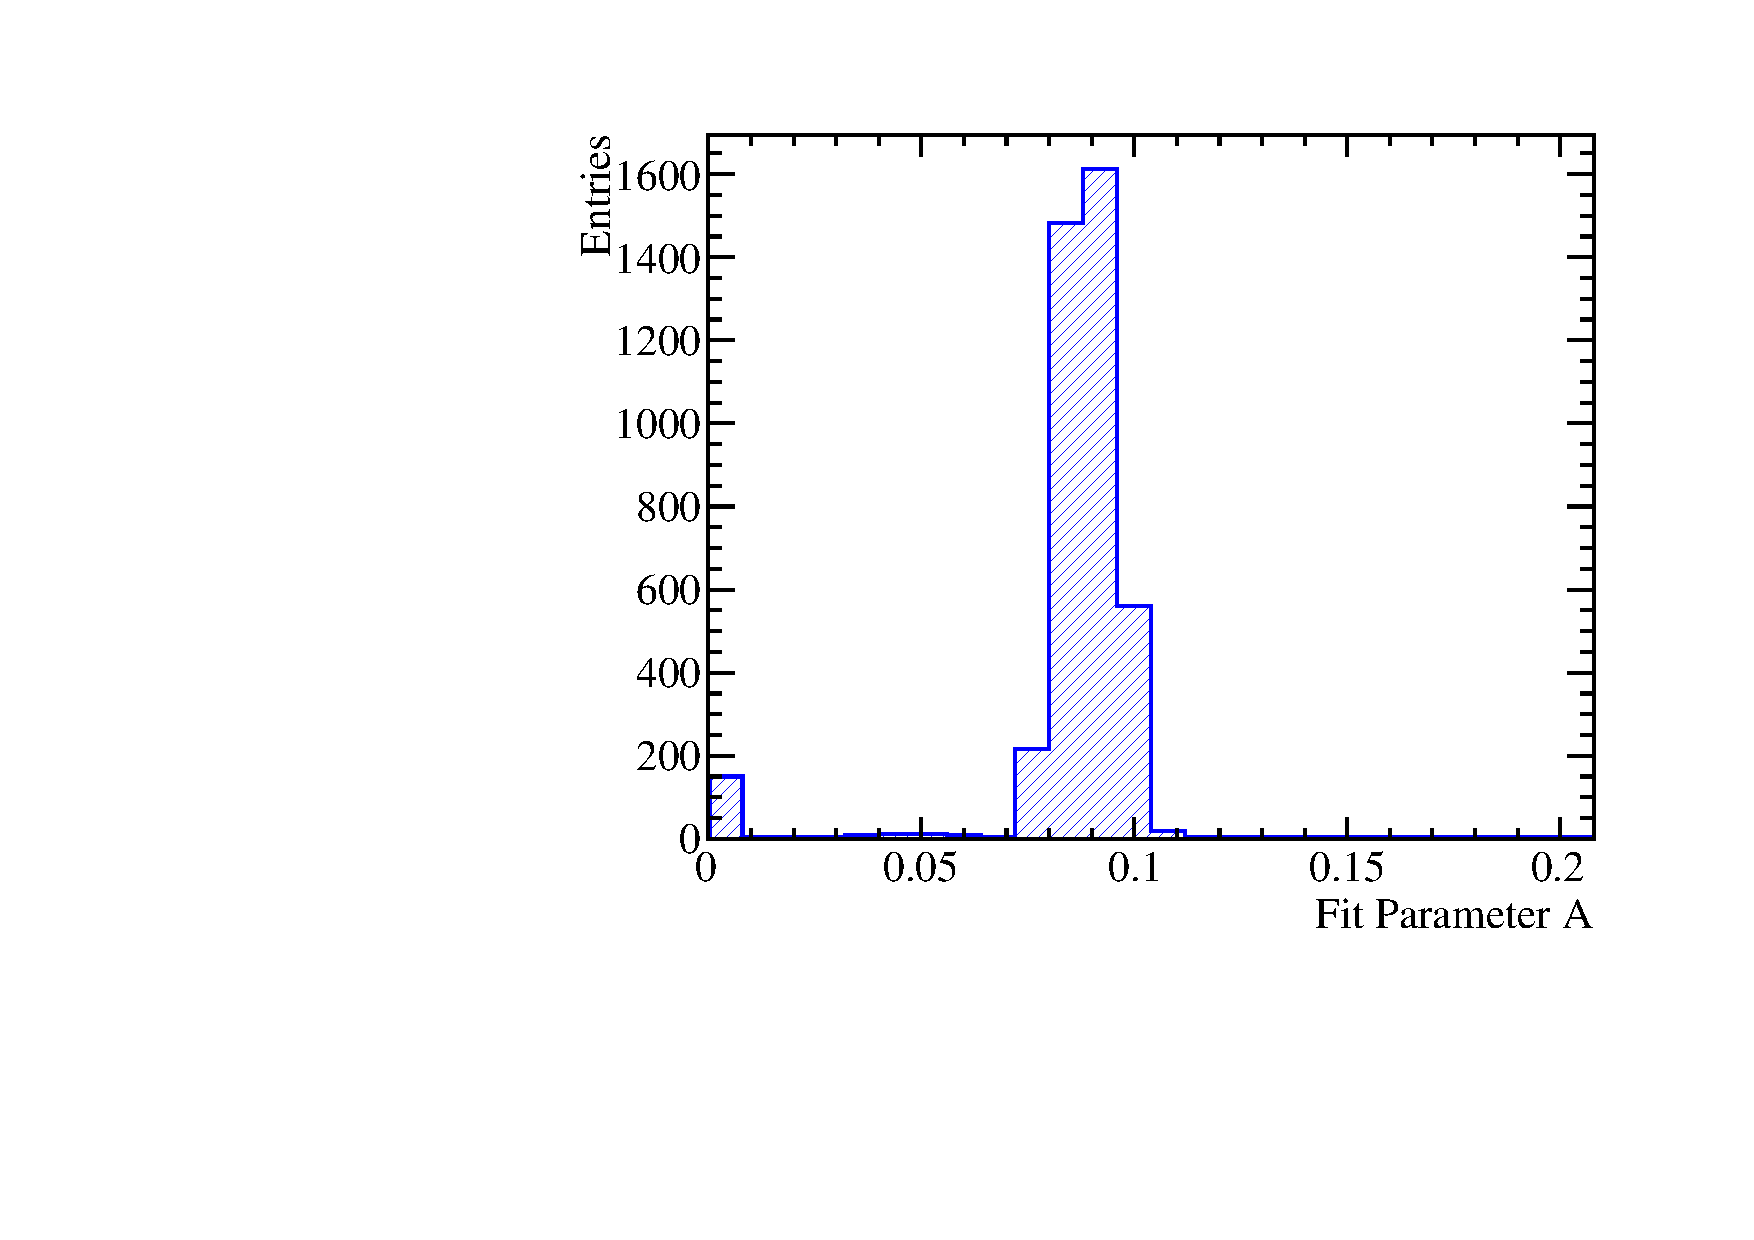
\includegraphics[width=0.5\textwidth]{CLICdpVertex/Plots/TestPulseCalibration/FitParam/OneDHistFitParamA_Set9.pdf}}
\subfloat[$b$ parameter.]{\label{fig:fitparams2}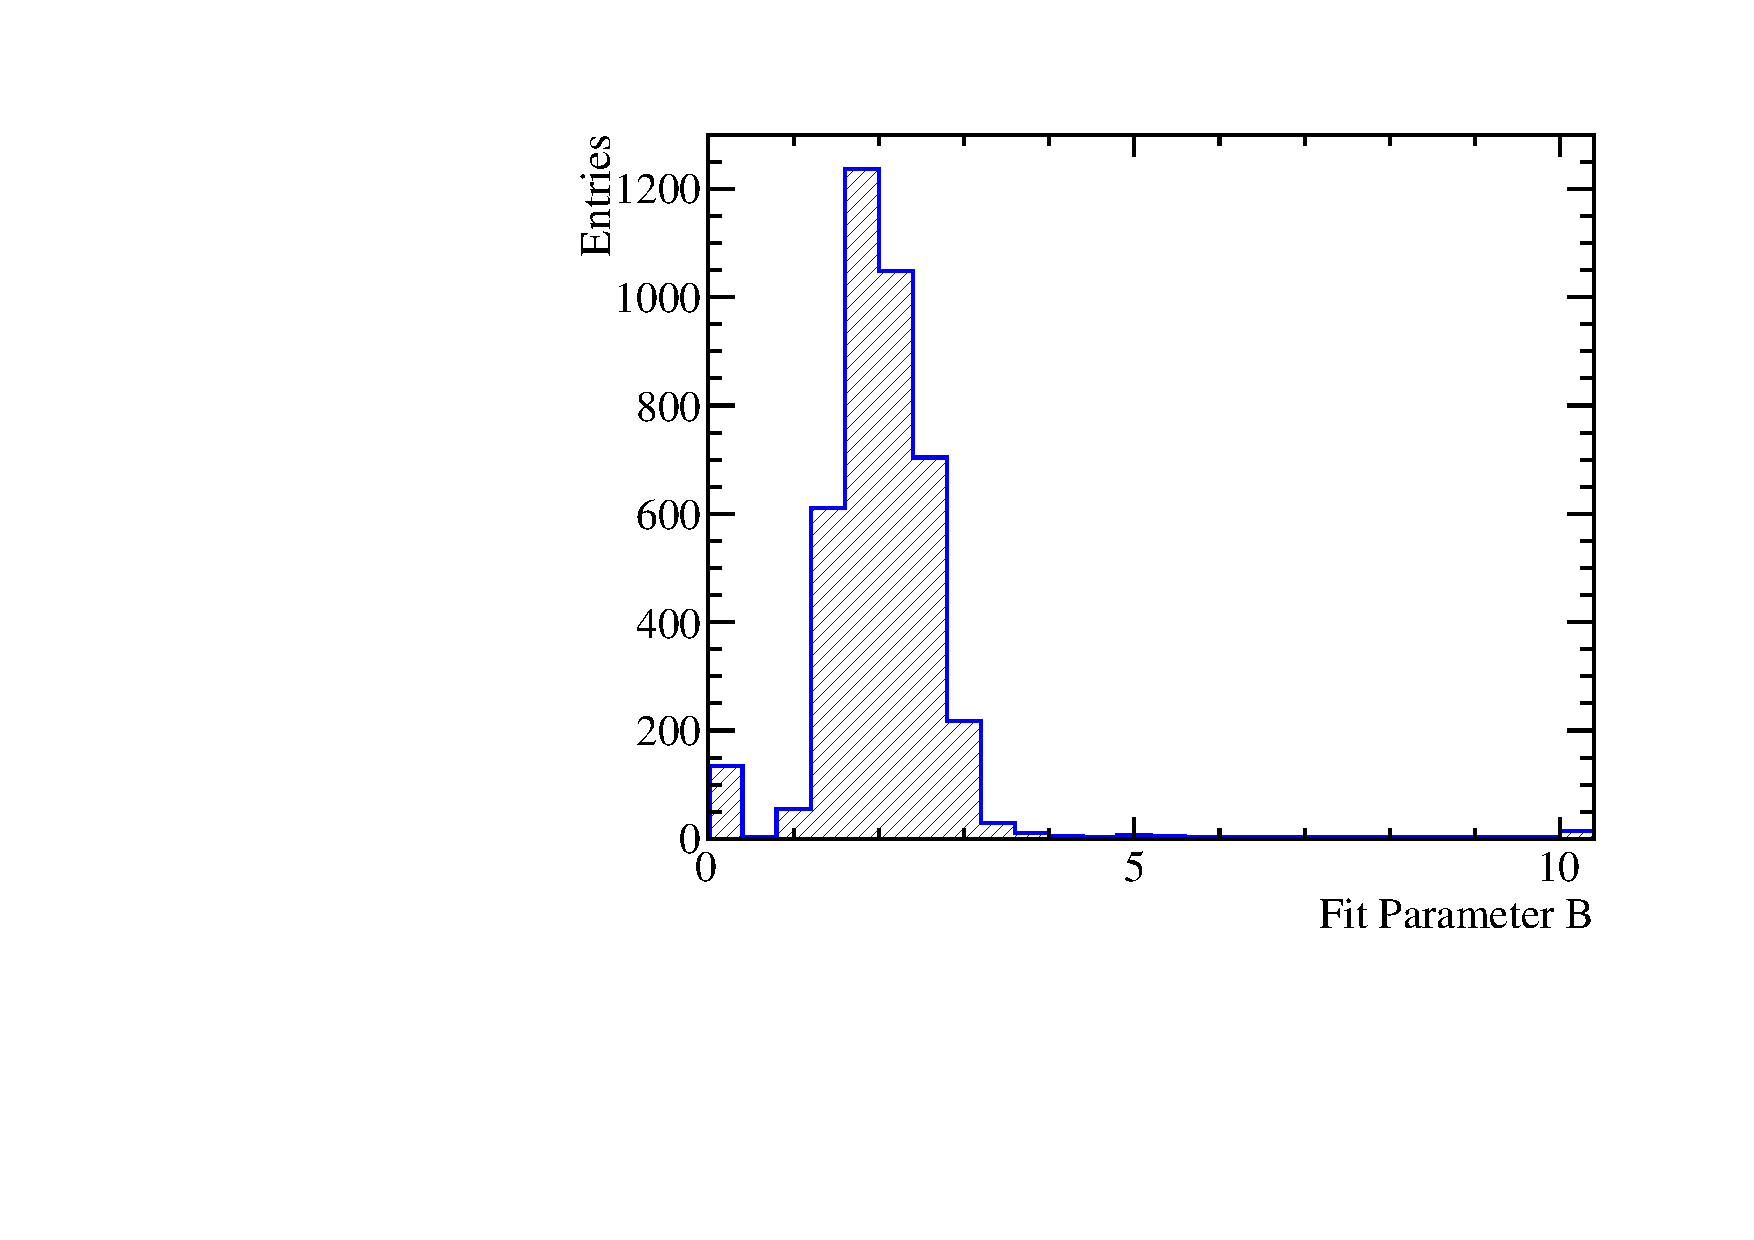
\includegraphics[width=0.5\textwidth]{CLICdpVertex/Plots/TestPulseCalibration/FitParam/OneDHistFitParamB_Set9.pdf}}\hfill
\subfloat[$c$ parameter.]{\label{fig:fitparams3}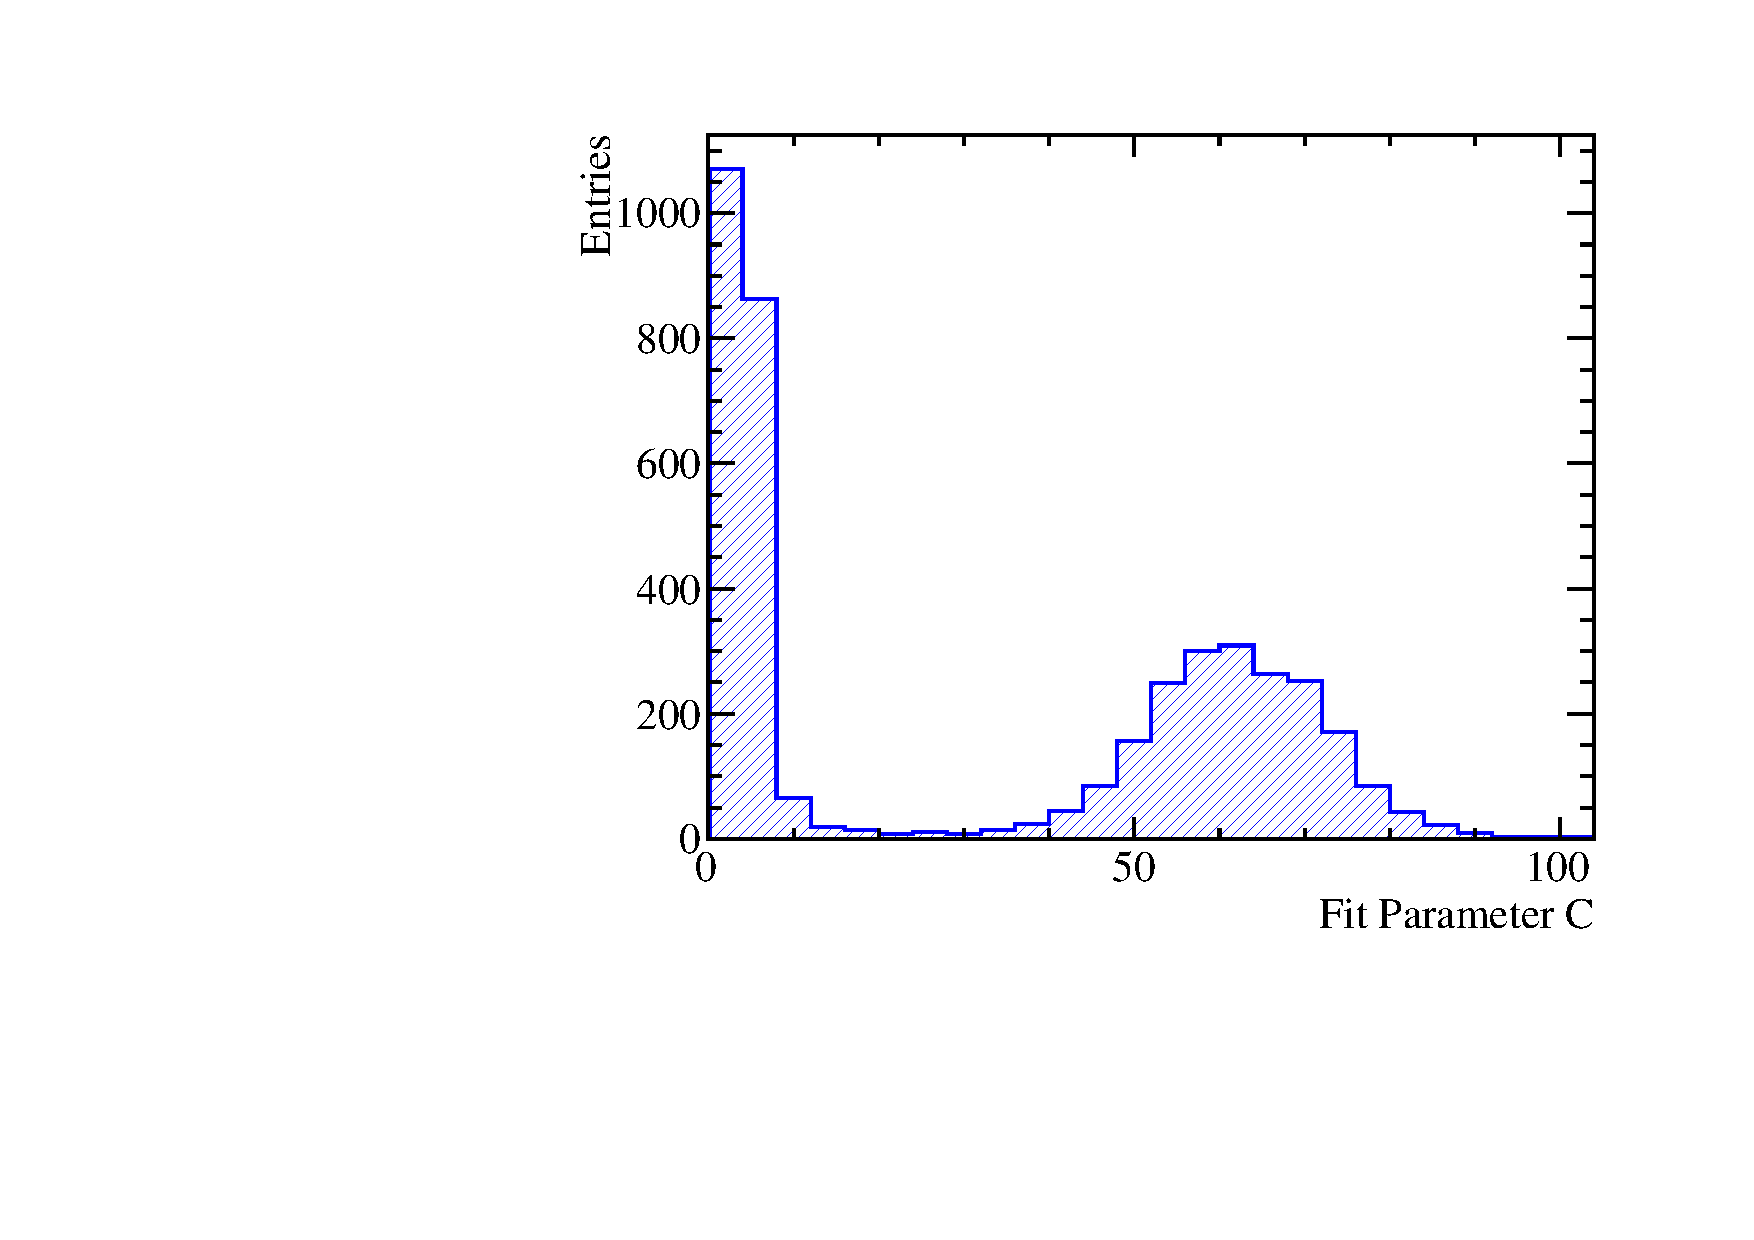
\includegraphics[width=0.5\textwidth]{CLICdpVertex/Plots/TestPulseCalibration/FitParam/OneDHistFitParamC_Set9.pdf}}
\subfloat[$t$ parameter.]{\label{fig:fitparams4}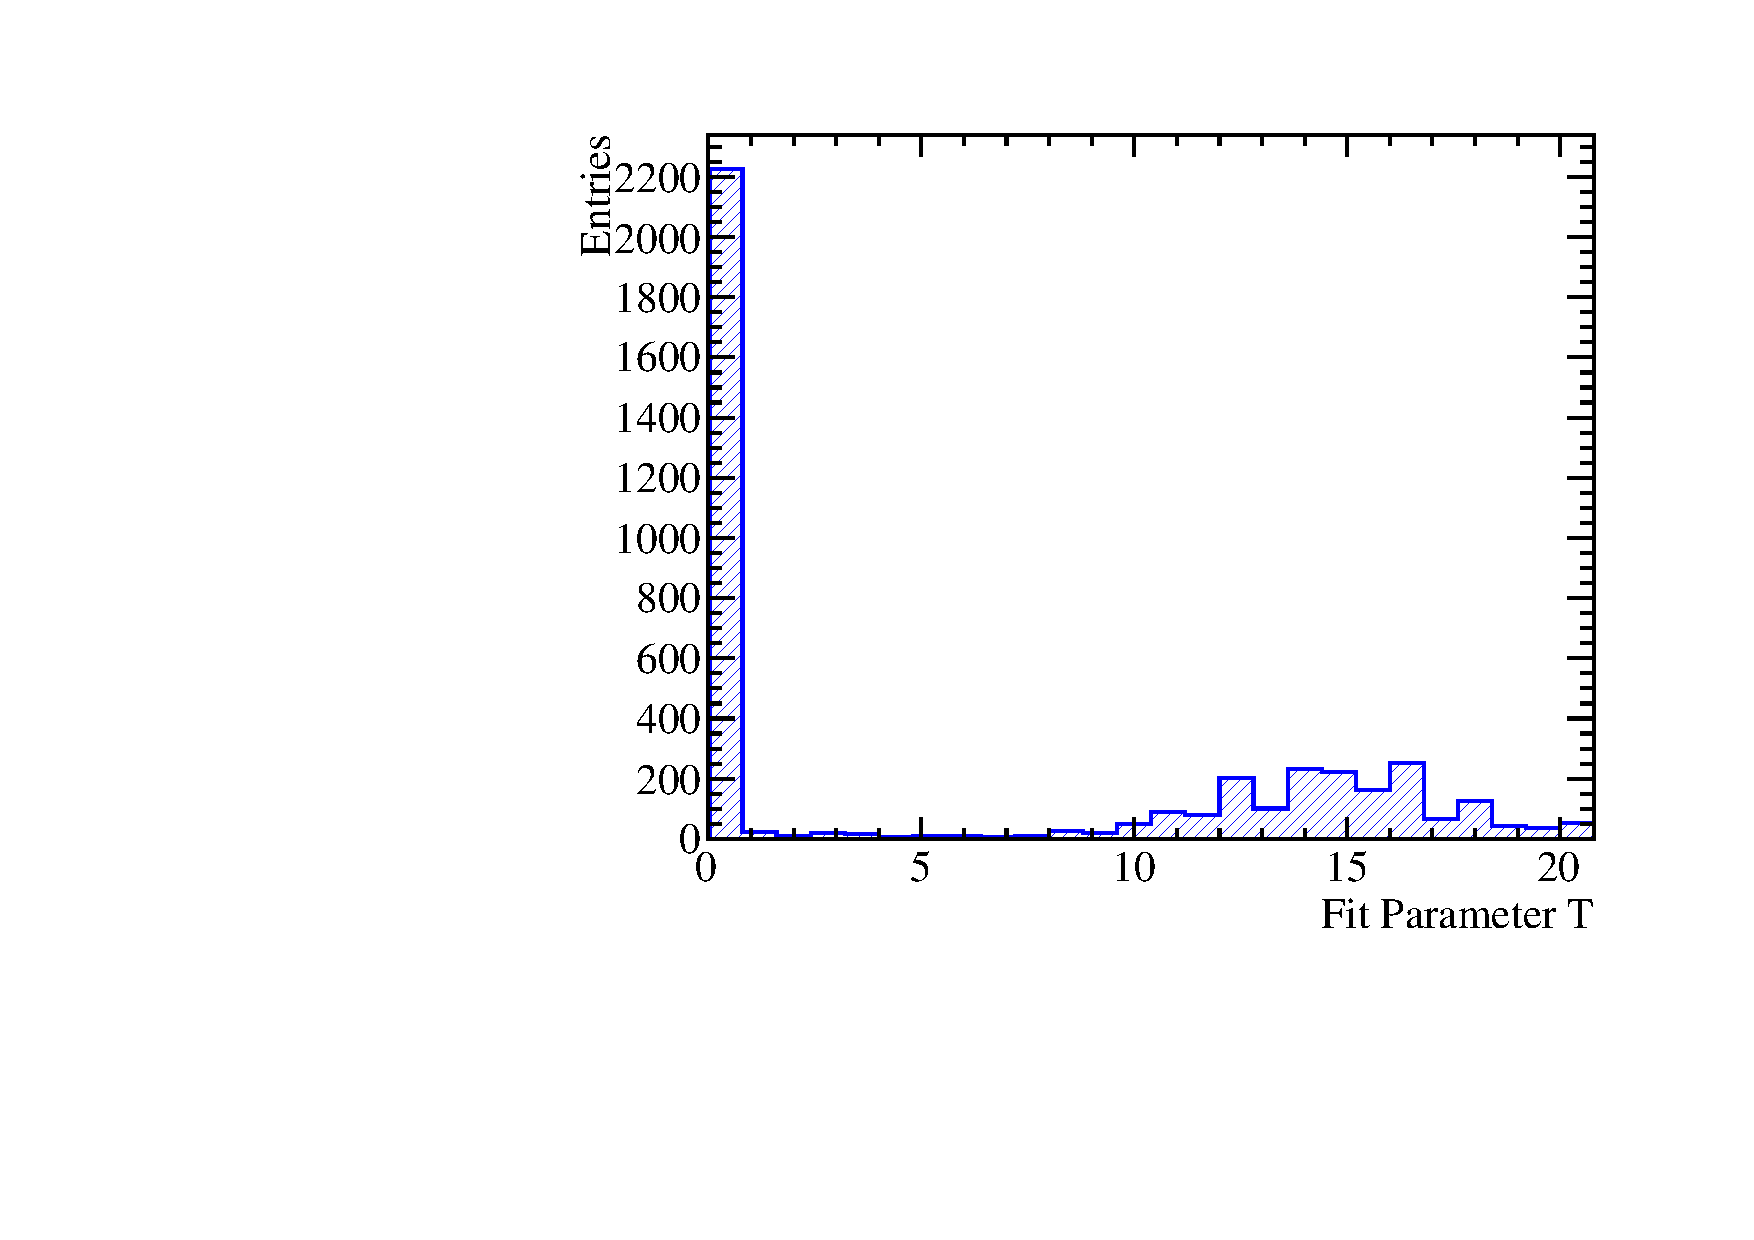
\includegraphics[width=0.5\textwidth]{CLICdpVertex/Plots/TestPulseCalibration/FitParam/OneDHistFitParamT_Set9.pdf}}
\caption[The distribution of the surrogate function parameters obtained when fitting the ToT as a function of injected pulse height for SET 9.  \protect\subref{fig:fitparams1}, \protect\subref{fig:fitparams2}, \protect\subref{fig:fitparams3} and \protect\subref{fig:fitparams4} show the distribution of the $a$, $b$, $c$ and $d$ parameters respectively.]{The distribution of the surrogate function parameters obtained when fitting the ToT as a function of injected pulse height for SET 9.  \protect\subref{fig:fitparams1}, \protect\subref{fig:fitparams2}, \protect\subref{fig:fitparams3} and \protect\subref{fig:fitparams4} show the distribution of the $a$, $b$, $c$ and $d$ parameters respectively.}  
\label{fig:fitparams}
\end{figure}

The peaks at zero in the distribution of the $a$ and $b$ parameters, containing $\approx$ 150 entries, correspond to noisy and dead pixels.  These damaged pixels will be found in the device due to problems occurring in the manufacturing process.  The majority of the $a$ and $b$ parameters are centred around a single value, which indicates a similar response in the linear region of the surrogate function, however, the $c$ and $t$ parameters are centred around one of two values.  When examining the distribution of these parameters as a function of position on the matrix, shown in figure \ref{fig:fitparams2d} for a selected device, it can be seen that the structure is related to the column a given pixel is in.  This feature is present in all devices considered and the underlying cause, the unwanted feedback capacitance, will be remedied in the next generation of the CLICpix ASIC.

\begin{figure}[h!]
\centering
\subfloat[$c$ parameter.]{\label{fig:fitparams2dc}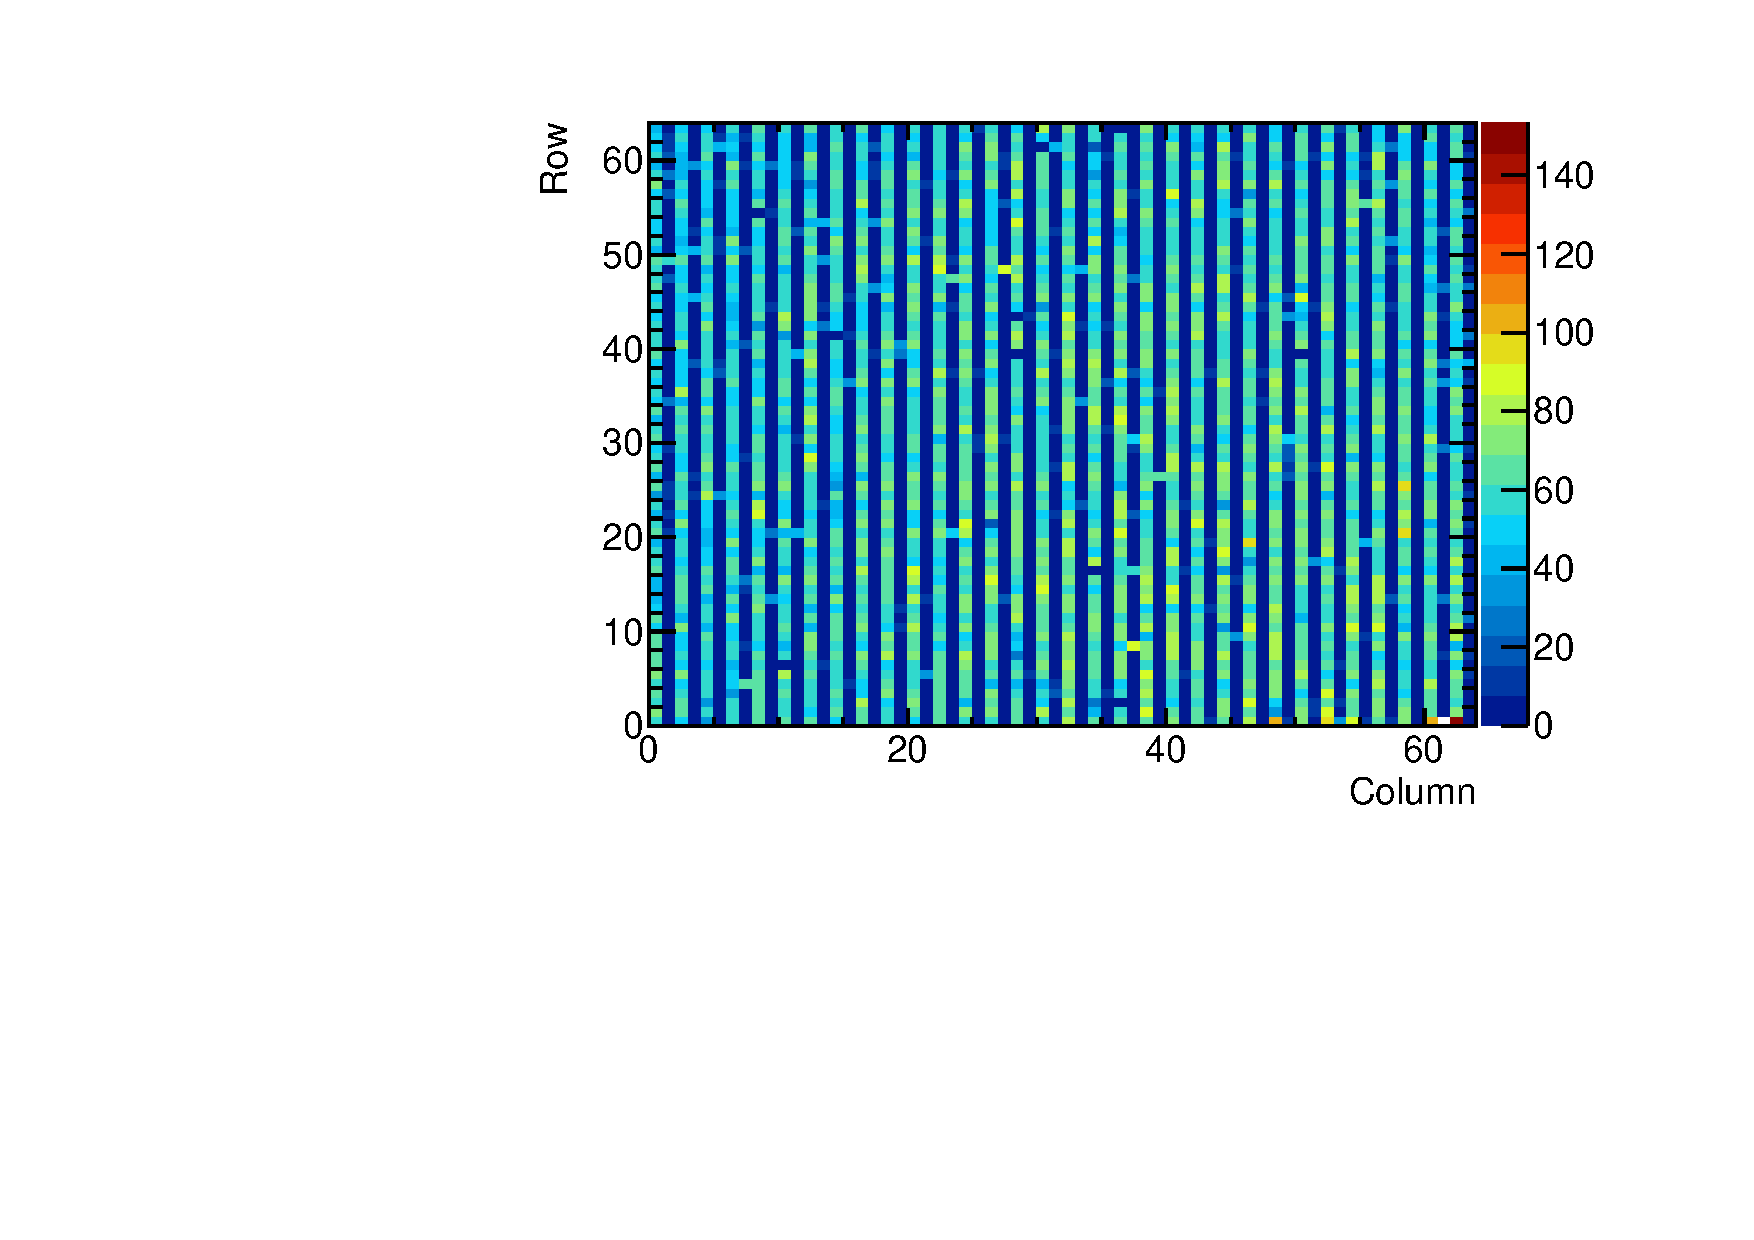
\includegraphics[width=0.5\textwidth]{CLICdpVertex/Plots/TestPulseCalibration/FitParam/FitParamC_Set9.pdf}}
\subfloat[$t$ parameter.]{\label{fig:fitparams2dt}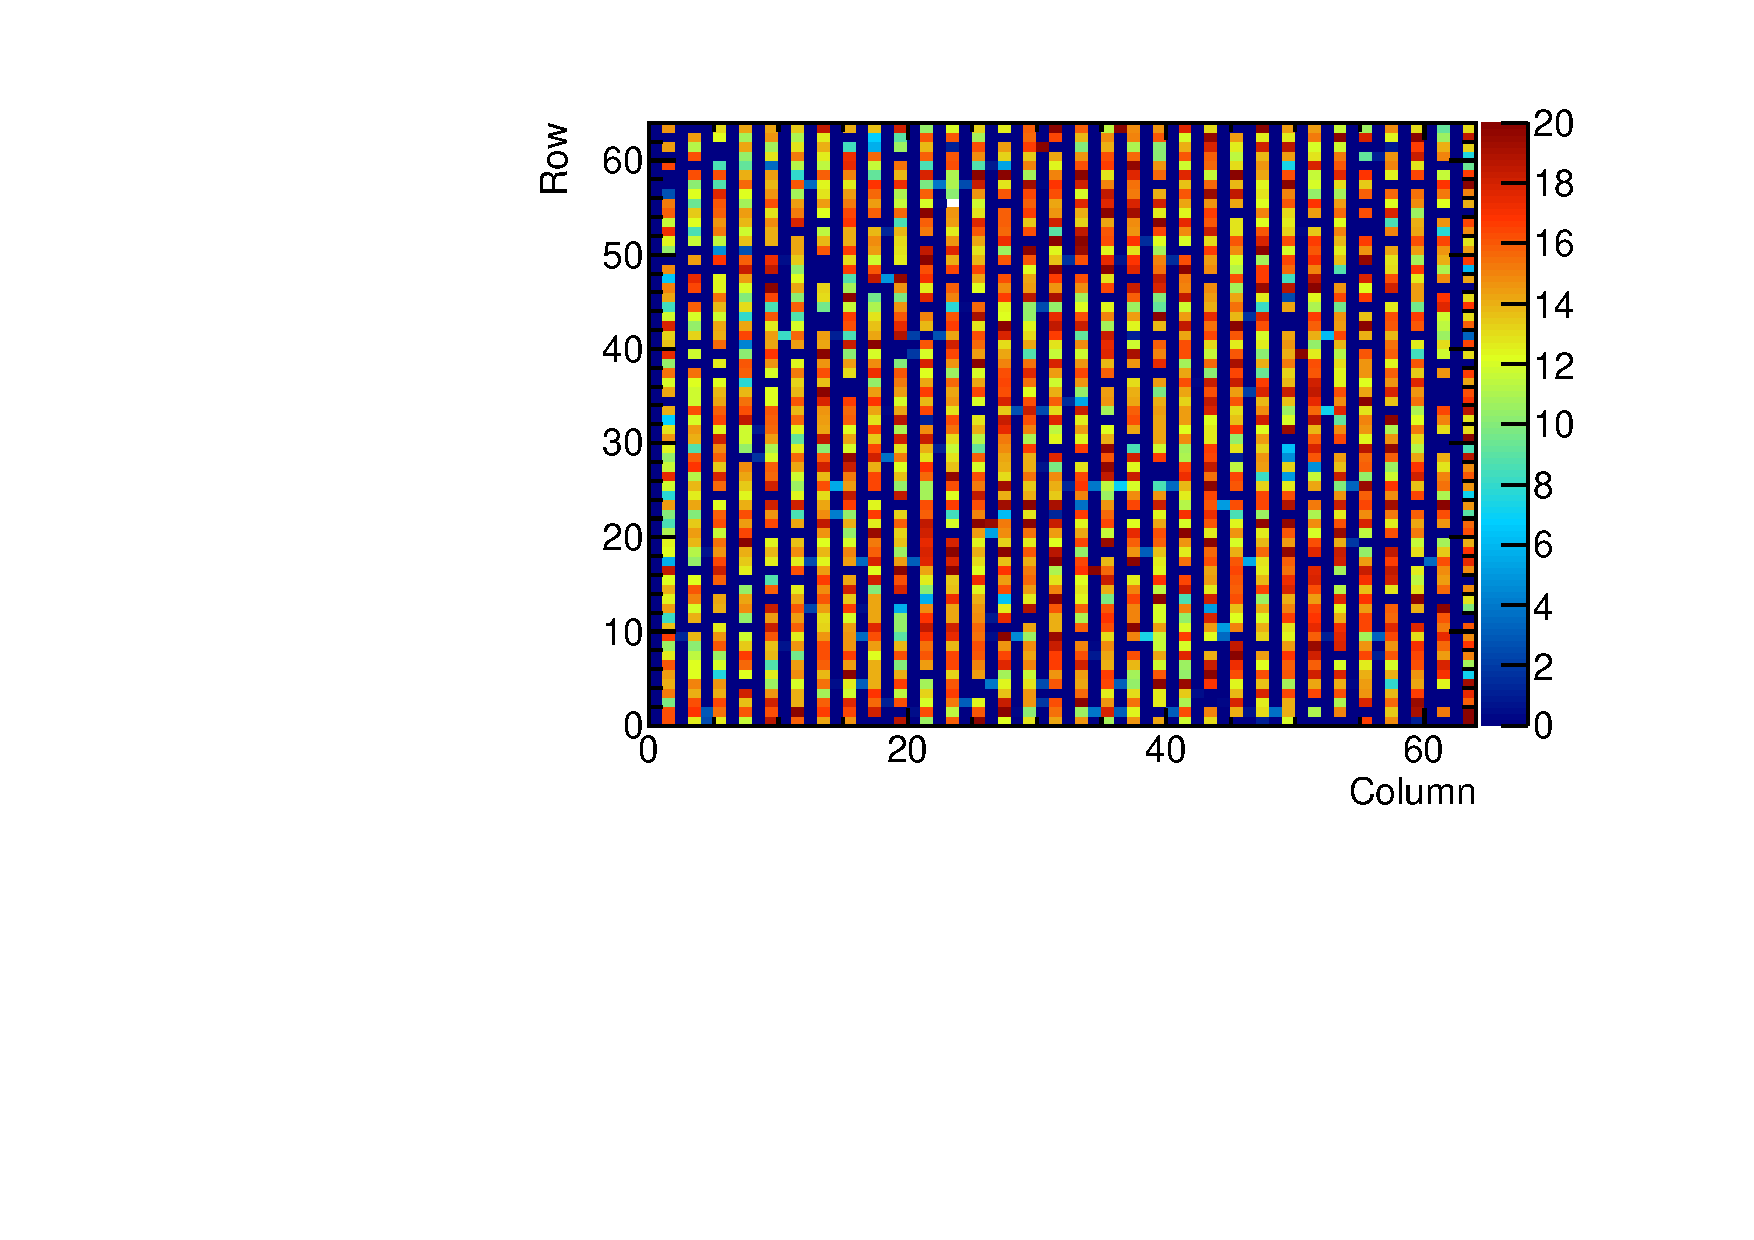
\includegraphics[width=0.5\textwidth]{CLICdpVertex/Plots/TestPulseCalibration/FitParam/FitParamT_Set9.pdf}}
\caption[The distribution of selected surrogate function parameters obtained when fitting the ToT as a function of injected pulse height for SET 9 as a function of matrix position.  \protect\subref{fig:fitparams2dc} and \protect\subref{fig:fitparams2dt} show the distribution of the $c$ and $t$ parameters respectively.]{The distribution of selected surrogate function parameters obtained when fitting the ToT as a function of injected pulse height for SET 9 as a function of matrix position.  \protect\subref{fig:fitparams2dc} and \protect\subref{fig:fitparams2dt} show the distribution of the $c$ and $t$ parameters respectively.}
\label{fig:fitparams2d}
\end{figure}

The matrix-averaged surrogate function fit parameters for all devices can be found in tables \ref{table:clicpixfitparamseven} and  \ref{table:clicpixfitparamsodd}, for the even and odd columns respectively.  The surrogate function for each device using these average parameters as input is shown in figure \ref{fig:testpulsemeanfit}.

\begin{table}[h!]
\centering
\begin{tabular}{ l r r r r}
\hline
Assembly & \multicolumn{1}{c}{$a$} & \multicolumn{1}{c}{$b$} & \multicolumn{1}{c}{$c$} & \multicolumn{1}{c}{$t$} \\ 
\hline
SET 9   & $0.0875 \pm 0.0005$ & $2.41 \pm 0.03$ & $5.1 \pm 0.1$ & $12.79 \pm 0.15$ \\
SET 10 & $0.0769 \pm 0.0005$ & $2.58 \pm 0.03$ & $7.5 \pm 0.2$ & $8.02 \pm 0.14$ \\
SET 12 & $0.0725 \pm 0.0005$ & $2.87 \pm 0.04$ & $12.1 \pm 0.3$ & $7.86 \pm 0.22$  \\
SET 13 & $0.0708 \pm 0.0005$ & $2.69 \pm 0.03$ & $16.2 \pm 0.3$ & $6.65 \pm 0.18$ \\
SET 15 & $0.0856 \pm 0.0005$ & $2.34 \pm 0.03$ & $5.1 \pm 0.2$ & $12.51 \pm 0.13$ \\
SET 16 & $0.0746 \pm 0.0004$ & $2.32 \pm 0.02$ & $13.7 \pm 0.3$ & $6.65\pm 0.16$ \\
\hline
\end{tabular}
\caption[The average fit parameters for even columns of CLICpix sensor.  The reported error was calculated using the standard error in the mean when averaging the fit parameters across the matrix.]{The average fit parameters for even columns of CLICpix sensor.  The reported error was calculated using the standard error in the mean when averaging the fit parameters across the matrix.}
\label{table:clicpixfitparamseven}
\vspace{\floatsep}
\centering
\begin{tabular}{ l r r r r}
\hline
Assembly & \multicolumn{1}{c}{$a$} & \multicolumn{1}{c}{$b$} & \multicolumn{1}{c}{$c$} & \multicolumn{1}{c}{$t$} \\ 
\hline
SET 9   & $0.0834 \pm 0.0003$ & $1.72 \pm 0.01$ & $61.0 \pm 0.3$ & $0.25 \pm 0.09$ \\
SET 10 & $0.0759 \pm 0.0002$ & $1.63 \pm 0.01$ & $43.2 \pm 0.2$ & $0.10 \pm 0.02$ \\
SET 12 & $0.0731 \pm 0.0003$ & $1.92 \pm 0.02$ & $51.5 \pm 0.3$ & $0.36 \pm 0.12$ \\
SET 13 & $0.0713 \pm 0.0002$ & $1.72 \pm 0.01$ & $52.5 \pm 0.3$ & $0.18 \pm 0.07$ \\
SET 15 & $0.0836 \pm 0.0003$ & $1.52 \pm 0.02$ & $52.7 \pm 0.3$ & $0.42 \pm 0.08$ \\
SET 16  & $0.0727 \pm 0.0002$ & $1.49 \pm 0.01$ & $50.7 \pm 0.2$ & $0.10 \pm 0.03$ \\
\hline
\end{tabular}
\caption[The average fit parameters for odd columns of CLICpix sensor.  The reported error was calculated using the standard error in the mean when averaging the fit parameters across the matrix.]{The average fit parameters for odd columns of CLICpix sensor.  The reported error was calculated using the standard error in the mean when averaging the fit parameters across the matrix.}\label{table:clicpixfitparamsodd}
\end{table}

\begin{figure}[h!]
\centering
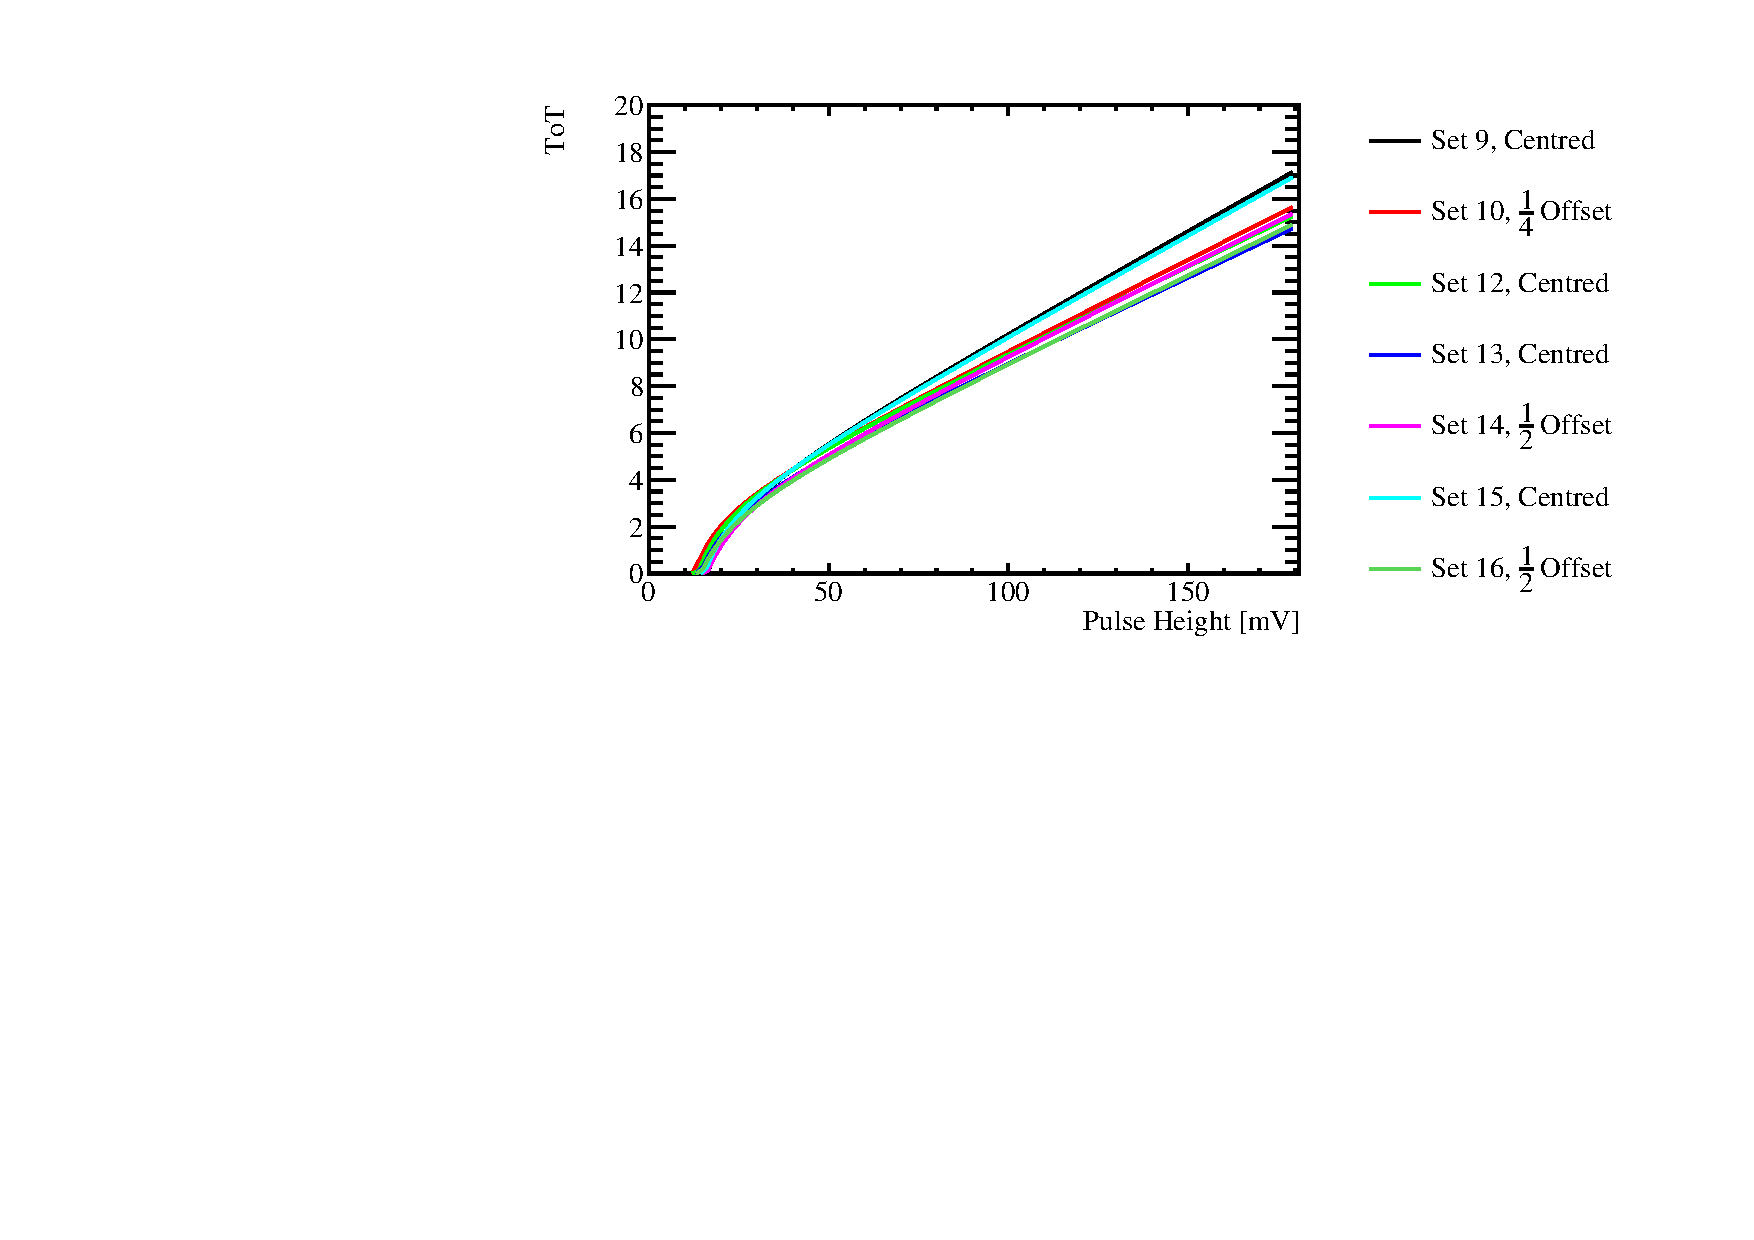
\includegraphics[width=1.0\textwidth]{CLICdpVertex/Plots/TestPulseCalibration/FitParam/AverageToT_vs_InjectedPulseHeight.pdf}
\caption[The average ToT response as a function of injected pulse height, which is represented using the surrogate function.  Parameters for the surrogate function are obtained by fitting the ToT against pulse height curve for all pixels in the matrix.  The results are divided into even and odd columns to account for the differing effective thresholds on alternate CLICpix columns.]{The average ToT response as a function of injected pulse height, which is represented using the surrogate function.  Parameters for the surrogate function are obtained by fitting the ToT against pulse height curve for all pixels in the matrix.  The results are divided into even and odd columns to account for the differing effective thresholds on alternate CLICpix columns.}
\label{fig:testpulsemeanfit}
\end{figure}

As figure \ref{fig:testpulsemeanfit} shows, the response of the CLICpix to the injected pulse height is largely uniform across all samples.  For all devices the turn-on pulse height is $\approx$ 10~mV and saturation, which occurs when the ToT output reaches the maximum value of 15, occurs at $\approx$ 150~mV.  The differing column structure exists due to the unwanted feedback capacitance between the discriminator output and amplifier input.  This unwanted feedback leads to a sharper rise in ToT for even-numbered columns than for odd-numbered columns, because, in effect, the even-numbered columns are operating at a lower threshold.  This column structure is present in all devices considered.  The uniformity of the response of the CLICpix ASICs observed in this study make comparisons between the misaligned samples clearer.  These results show that any performance differences observed between the misaligned devices do not originate from the intrinsic behaviour of the CLICpix ASIC.   

%========================================================================================
%========================================================================================

\section{Test Beam Analysis}
\label{sec:testbeam}
Test beam measurements were used to characterise the behaviour of the prototype capacitively coupled pixel detectors.  These measurements are particularly useful as they include information relating to the properties of the particles passing through the device under test (DUT).  This information is crucial for calculating the efficiency of the devices, which will ultimately determine whether the device is fit for use in the CLIC vertex detector.  

The trajectory of any particles passing through the DUT was measured in the test beam setup using a telescope.  The telescope consisted of several planes of pixel detectors mounted either side of the DUT.  As low energy particles would be stopped by the telescope detector planes, telescopes can only be used to measure the trajectory of relatively high energy particles.  This means that they cannot be used in lab based measurements, but can be used in test beams where high energy particles can be safely produced.  

%========================================================================================

\subsection{Test Beam Setup}
Test beam experiments were carried out in August and September 2015 on the H6 beam line in the CERN SPS North Area.  The beam consisted of positively charged hadrons of momenta 120 GeV/c.  Mean particle rates of 500 kHz/cm$^{2}$ were observed during the 4.8~s spills at intervals of 25~s. The devices under test were mounted on an EUDET/AIDA telescope \cite{Rubinskiy:2000287}.  This telescope consisted of six planes of sensors, three on either side of the DUT, constructed of Mimosa pixel detectors.  This telescope provided a resolution of 1.6 $\micro$m on the intercept position between tracks passing through the device and the DUT mounted on it.  

%========================================================================================

\subsection{Analysis}
A number of cuts were applied to veto the effect of noisy pixels and tracks that underwent non-negligible multiple scattering \cite{Tehrani:2016ogb}.  These effects would lead to discrepancies in the reported efficiencies of the devices, which are not representative of the true device performance.  Any pixels identified on the DUT that were deemed to be noisy were removed from the analysis.  A pixel was deemed noisy if it responded at a mean rate greater than 5 $\sigma$ in comparison to the average rate across the whole matrix.  In addition to this, any tracks with an intercept on the DUT within half a pixel width of a noisy pixel were also rejected from the analysis.  As tracks may undergo non-negligible multiple scattering, a $\chi^{2}$ cut was used to remove less precisely reconstructed tracks.  Furthermore, all tracks occurring within 125 $\micro$m of each other were vetoed, in order to reduce the possibility of mis-association of clusters to tracks. 

After the application of these cuts, the track position on the DUT was calculated using the measured particle trajectory through the telescope planes.  This was followed by a search around the intercept position on the DUT to find an associated cluster.  Clusters were associated to the track if they fell within 75 $\micro$m, or 3 pixels, about the intercept position.  If multiple clusters were associated to a track the cluster position was calculated as the ToT-weighted centre-of-gravity.  

Alignment of the telescope planes was essential for ensuring that the correct trajectory of the particles passing through the setup could be determined.  Furthermore, alignment of the DUT with respect to the telescope planes was critical for ensuring the correct track intercept position was found.  With that in mind the six telescope planes were aligned by minimising the total track $\chi^{2}$ with respect to the global alignment parameters.  The tracks that were created in the alignment procedure are referred to as "rough tracks" since they are produced using the hits from sensor planes that may not be ideally aligned.  The alignment proceeded by one telescope plane at a time until all planes were accounted for.  This procedure was iteratively repeated, updating the global alignment parameters to the optimal values found each time, until no further gains could be made.  Once the telescope planes were aligned, the DUT was aligned in a similar manner, but this time minimising the root mean squared of the residual distribution.  Here, residuals are defined as the distance between the track intercept and associated cluster centre-of-gravity on the DUT.  

%========================================================================================

\subsection{Results}
The metric used for characterising the device performance in the test beam is the single hit efficiency, $\epsilon$.  This is defined as the number of tracks with associated clusters recorded by the DUT, $n$, divided by the number of reconstructed tracks passing through the DUT recorded by the telescope, $m$. The errors shown on the efficiency measurements are given by $\sqrt{\epsilon (1 - \epsilon)/m}$, which follows from the variance of $n$ given binomial statistics with mean $\epsilon$.  The single hit efficiency as a function of threshold for all devices is shown in figure \ref{fig:efficiency}.  The threshold, in units of number of electrons, is the size of the signal that must be injected into the CLICpix ASIC to generate a hit. 

\begin{figure}
\centering
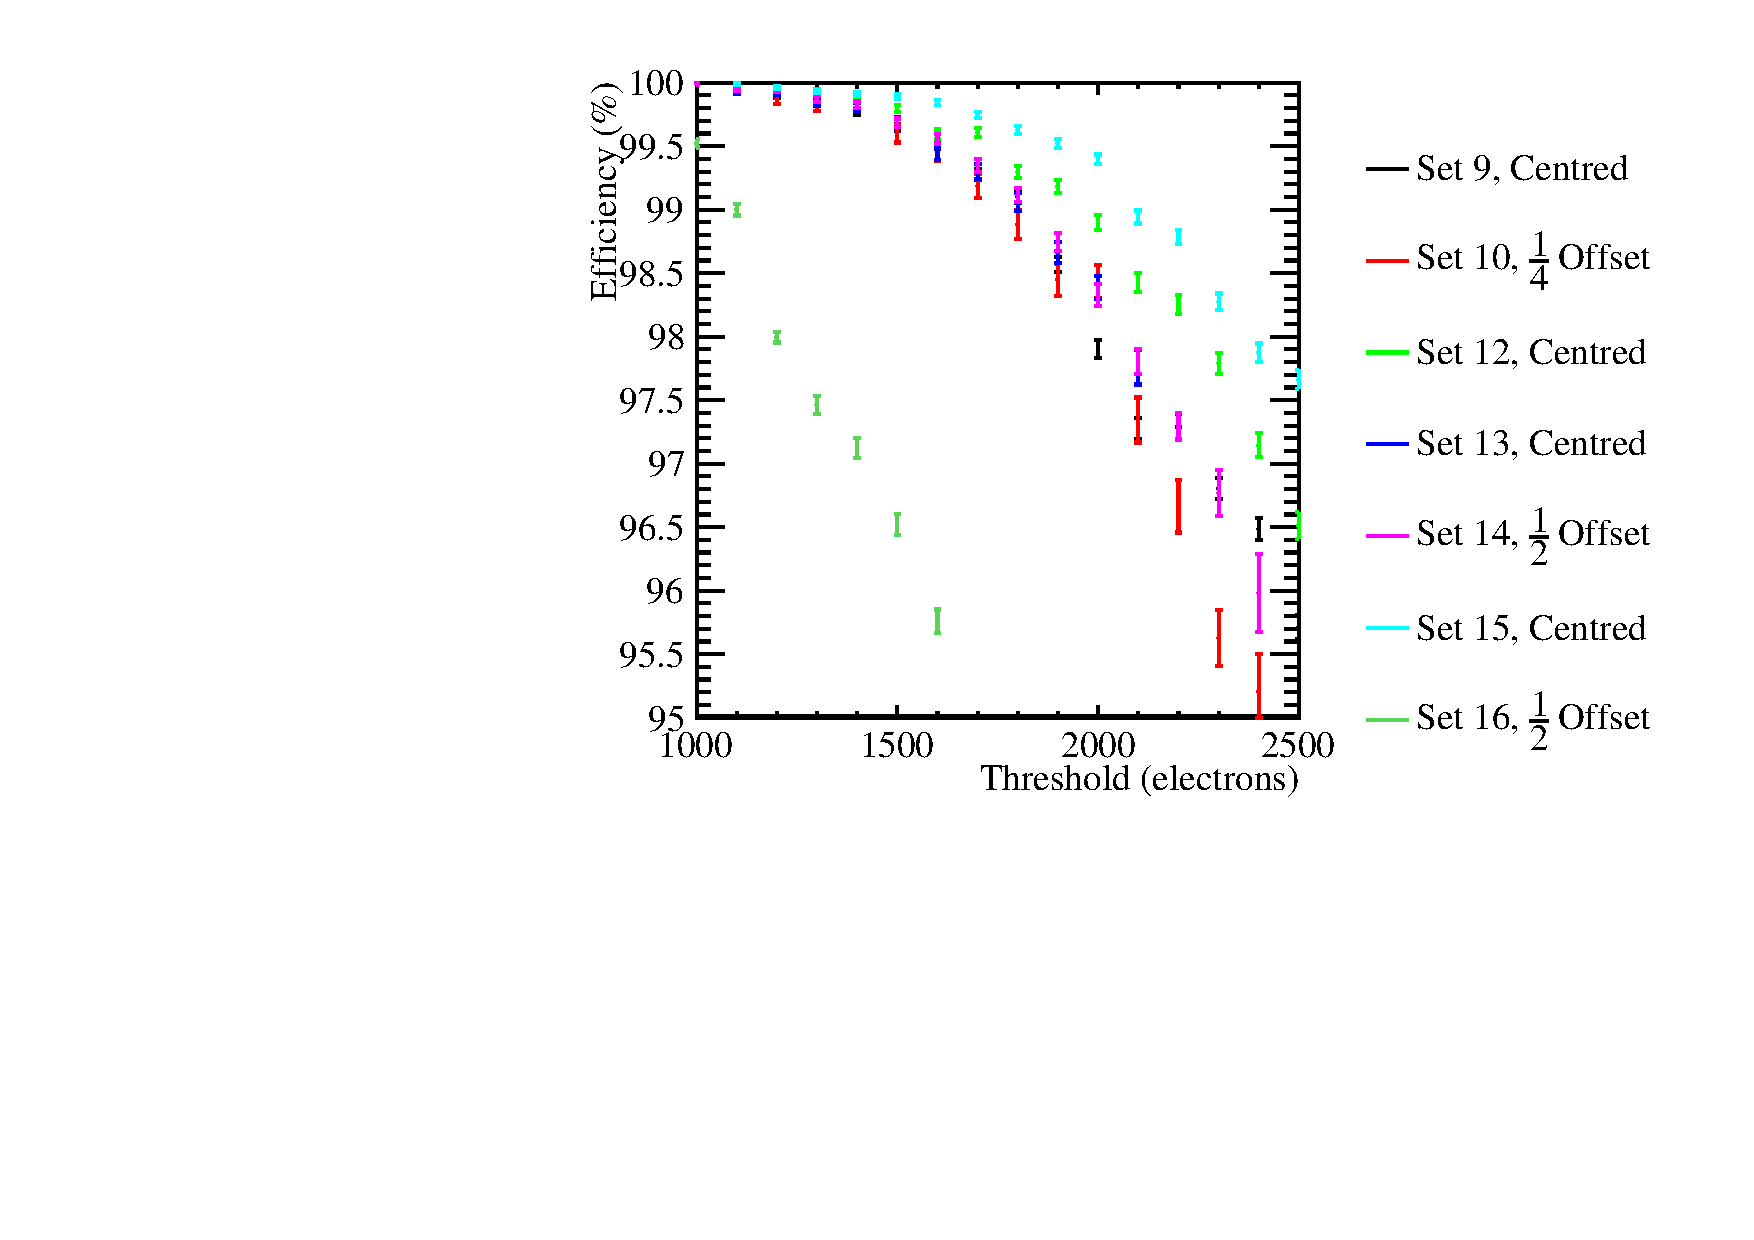
\includegraphics[width=1.0\textwidth]{CLICdpVertex/Plots/TestBeamData/EfficiencyThresholdPlot.pdf}
\caption[The efficiency of the devices considered as a function of the threshold applied.]{The efficiency of the devices considered as a function of the threshold applied.}
\label{fig:efficiency}
\end{figure}

The data indicates that for all assemblies the single hit efficiency of the detector decreases when a higher amount of charge is required to generate a signal, which is to be expected.  However, the efficiency of all samples, with the exception of the $\frac{1}{2}$-offset sample, is still above 99\% up to a threshold of 2000 electrons.  This is encouraging behaviour as the larger the threshold that can be applied, the lower the effects from noise will be.  Reducing the effects from noise will aid tracking performance in the CLIC vertex detector, which is highly desirable.  It is clear that the $\frac{1}{2}$ offset sample, SET 16, has a much lower efficiency as a function of threshold in comparison to the other samples.  For the same deposited charge in the CCPDv3 the $\frac{1}{2}$-offset sample will, due to the reduced capacitance, produce a smaller signal in the CLICpix than the centred samples.  This is the cause of the reduced efficiency as a function of threshold in this sample.  More encouragingly is the behaviour of the $\frac{1}{4}$-offset sample, SET 14, which in terms of performance is comparable to the aligned samples.  There is a degradation in efficiency of the $\frac{1}{4}$-offset sample with respect to the aligned sampled, which is to be expected given the reduced capacitance, however, it is relatively small.  These results indicate that even with a relatively large misalignment between the CCPDv3 and CLICpix pads the device performance is not significantly affected, and therefore manufacturing tolerances of $\frac{1}{4}$ of a pixel width would not be problematic if this device were used for the CLIC vertex detector.

%========================================================================================

\section{Conclusions}
In summary, for the capacitively coupled pixel detectors considered in this analysis:

\begin{itemize}
\item The CCPDv3 sensor ASIC properties have been characterised and were found to be comparable across all devices.
\item A calibration of the CLICpix readout ASIC was performed and their behaviour was found to be comparable across all devices.  
\item When combining the CCPDv3 and CLICpix characterisations, it becomes clear that any performance differences between the devices are due to the capacitive coupling gluing layer as opposed to the intrinsic behaviour of the ASICs.
\item Test beam analysis of the devices found that device fabrication tolerances of up to $\frac{1}{4}$ of a pixel width would not harm the performance of these devices should they be used for the CLIC vertex detector.  
\end{itemize}

%========================================================================================
